\documentclass[11pt]{article}
\usepackage[a4paper,margin=1.15in]{geometry}

\usepackage[T1]{fontenc}
\usepackage[utf8]{inputenc}
\usepackage{amsmath,amssymb,mathtools,amsthm,bm}
\usepackage{enumerate}
\usepackage{tikz}
\usepackage{float}
\usepackage{graphicx}
\usepackage[bookmarks=false]{hyperref}
\hypersetup{colorlinks=true,linkcolor=blue,citecolor=blue,urlcolor=blue,
  pdftitle={Braid Monodromy of Analytic Matrix Families: Sharp Discriminant Constants and Torus Extensions},
  pdfauthor={Chao Ma}}

\newtheorem{theorem}{Theorem}[section]
\newtheorem{proposition}[theorem]{Proposition}
\newtheorem{lemma}[theorem]{Lemma}
\newtheorem{corollary}[theorem]{Corollary}
\newtheorem{definition}[theorem]{Definition}
\newtheorem{example}[theorem]{Example}
\newtheorem{remark}[theorem]{Remark}
\newtheorem{convention}[theorem]{Convention}
\newtheorem{conjecture}[theorem]{Conjecture}

\numberwithin{equation}{section}
\DeclareMathOperator{\Conf}{Conf}
\DeclareMathOperator{\UConf}{UConf}
\DeclareMathOperator{\Disc}{Disc}
\DeclareMathOperator{\Res}{Res}
\DeclareMathOperator{\tr}{tr}
\DeclareMathOperator{\diag}{diag}
\DeclareMathOperator{\dist}{dist}
\DeclareMathOperator{\spec}{spec}
\DeclareMathOperator{\sgn}{sgn}
\newcommand{\bbC}{\mathbb C}
\newcommand{\bbR}{\mathbb R}
\newcommand{\bbD}{\mathbb D}
\newcommand{\bbP}{\mathbb P}
\newcommand{\bbZ}{\mathbb Z}
\newcommand{\bbQ}{\mathbb Q}
\newcommand{\bbT}{\mathbb T}
\newcommand{\cB}{\mathcal B}
\newcommand{\cC}{\mathcal C}
\newcommand{\cD}{\mathcal D}
\newcommand{\cE}{\mathcal E}
\newcommand{\cG}{\mathcal G}
\newcommand{\cP}{\mathcal P}
\newcommand{\cS}{\mathcal S}
\newcommand{\cT}{\mathcal T}
\newcommand{\norm}[1]{\left\|#1\right\|}
\newcommand{\abs}[1]{\left|#1\right|}
\newcommand{\ii}{\mathrm i}
\newcommand{\eps}{\varepsilon}
\newcommand{\pe}{\operatorname{pe}}
\newcommand{\wt}[1]{\widetilde{#1}}

\begin{document}


\title{Braid Monodromy of Analytic Matrix Families:\\Sharp Discriminant Constants and Torus Extensions}
\author{Chao Ma\\
Independent Researcher, London, United Kingdom\\
\texttt{raymond.ma@me.com}\\
ORCID: 0009-0004-2456-9098}
\date{}
\maketitle

\begin{abstract}
To an analytic family of $n\times n$ matrices with generically simple spectrum,
each loop in the parameter space assigns a conjugacy class in the braid group $B_n$
via the eigenvalue monodromy.  We develop a finite, operator-norm certificate
for this assignment: a positive discriminant margin on a compact based graph,
together with a sharp Lipschitz constant for the characteristic discriminant,
yields an explicit perturbation radius within which every generator braid
and every relation among them is stable.

The sharp Lipschitz constants are computed exactly in the quadratic and
traceless cubic cases.  The exact operator-norm Lipschitz constant for the
discriminant is $8R$ on the $2\times2$ ball and $162R^5$ on the traceless
$3\times3$ ball of radius $R$; both are attained by unit-root diagonal
families.  A roots-of-unity identity shows that the pattern
$n^{n+1}(n-1)R^{n(n-1)-1}$, proved here for \(n\in\{2,3\}\), is the natural
candidate for all \(n\).  For \(n=4\) we prove the sharp constant
\(3072R^{11}\).  The non-normal part is reduced to a finite four-point
Blaschke--Pick certificate; all regular strata are covered by the listed
analytic/Bernstein certificates, and the only hard Bernstein corner is closed
by an exact rational blow-up certificate supplied as a reproducible
supplementary proof object.

Three families illustrate the certificate with complete braid computations.
For the companion cubic $E^3-3E-k$, the two-puncture monodromy representation
surjects onto $B_3$ with kernel the normal closure of the Artin relation.
For $E^3-k^3-1$, the image is the cyclic group $\langle\sigma_1\sigma_2\rangle$.
On the two-dimensional Brillouin torus $\bbT^2$, we prove that families of
the form $H=g(k_1,k_2)M$ with $M=\mathrm{diag}(1,\omega,\omega^2)$ always
have braid monodromy valued in the centre $Z(B_3)$: rigid rotation of the
eigenvalue triangle forces every loop to map to a power of the full twist
$(\sigma_1\sigma_2)^3$.  Explicit Zariski--van Kampen computations determine
the representations on $\pi_1(\bbT^2)$ and $\pi_1(\bbT^2\setminus C)$
for specific two-parameter families, and a quartic $A_3$ arrangement
provides a $B_4$-valued example with explicit certified radius.
\end{abstract}

\noindent\textbf{Keywords:} braid monodromy; exceptional point; discriminant
complement; matrix family; configuration space; non-Hermitian matrix;
Nevanlinna--Pick interpolation.

\medskip
\noindent\textbf{MSC 2020:} 15A18, 20F36, 30C15, 14H30, 55R80, 81Q12.

\bigskip


%% ===================================================================
\section{Introduction}
%% ===================================================================

A matrix loop with simple spectrum determines a braid of its eigenvalues.  A
multi-parameter family determines a representation
\[
  \beta_H:\pi_1(\cP\setminus\cD,p_0)\longrightarrow B_n
\]
from the complement of the repeated-eigenvalue locus.  The aim of this paper
is to make such representations certifiable when the family is known only
through finitely many matrix samples on selected loops.

The question is natural in non-Hermitian spectral theory.  Exceptional points
are eigenvalue branch points, and loops around them carry braid charges
\cite{Heiss2012,Ozdemir2019,Bergholtz2021,Ding2022,Carlstrom2018,Wojcik2020,Patil2022}.
Thus a physical spectral motion is converted into a word in an Artin braid
group, while the arrangement of exceptional points supplies the discriminant
complement on which the word is read.  Numerically, however, the loop is a
mesh, not a continuum.  One has to know that the graph stays off the
discriminant between samples, and that small matrix errors do not change the
braid word or the relations among several chosen loops.

The certificate uses only elementary homotopy and a Lipschitz estimate.  The
unordered spectrum maps the discriminant complement to \(\UConf_n(\bbC)\).
On a compact based graph \(G\), a positive margin \(M_G\) for the
characteristic discriminant keeps the straight-line homotopy from a family to
a nearby family inside configuration space, provided the perturbation is
smaller than the associated operator-norm radius.  Hence the generator braids
carried by \(G\) are fixed simultaneously.  If only a mesh is available, the
observed margin is reduced by the explicit correction \(\cG(R_*)L_Gh_G\).

Section~\ref{sec:config} fixes the configuration-space conventions.
Section~\ref{sec:tr0constant} proves the quantitative input used later: for
trace-zero cubic matrices \(\cG_{\tr=0,3}(R)=162R^5\), while for trace-zero
quartic matrices it proves the sharp constant \(3072R^{11}\), with the
non-normal reduced Pick certificate supplied in the appendix and accompanying
supplementary proof object.  The graph,
sampling, and adaptive gap certificates occupy
Sections~\ref{sec:graph}--\ref{sec:adaptive}.  The examples separate two
cubic arrangements with the same local degree-three flavour but different
global monodromy.  The companion cubic \(E^3-3E-k\) gives a surjection onto
\(B_3\), whereas the factorised family \(E^3-k^3-1\) has cyclic image
generated by \(\sigma_1\sigma_2\).  Section~\ref{sec:local-models} relates these computations
to the cusp and to a quartic \(A_3\) benchmark.
Section~\ref{sec:torus} extends the graph certificate to the
two-dimensional Brillouin torus \(\bbT^2\): the discriminant locus is
generically a finite set of isolated exceptional points (complex-valued
\(\Delta\)) or an embedded curve (real-valued \(\Delta\)), and two
versions of the stability theorem cover the cases \(M_{\bbT^2}>0\) and
\(C\neq\varnothing\) separately.
Proposition~\ref{prop:T2-no-puncture} and
Proposition~\ref{prop:T2-degenerate-three-zero}
work out explicit families \(H=gM\) whose braid monodromy maps
\(\pi_1(\bbT^2)\) and \(\pi_1(\bbT^2\setminus C)\) into the centre
\(Z(B_3)\), with complete Zariski--van Kampen verification.


%% ===================================================================
\section{Configuration spaces and spectral braid monodromy}\label{sec:config}
%% ===================================================================

Let
\[
  \Conf_n(\bbC)=\{(z_1,\ldots,z_n)\in\bbC^n:z_i\ne z_j\text{ for }i\ne j\}
\]
be the ordered configuration space and let
\[
  \UConf_n(\bbC)=\Conf_n(\bbC)/S_n
\]
be the unordered configuration space.  The braid group is
\[
  B_n=\pi_1(\UConf_n(\bbC),Q_0),
\]
where $Q_0$ is a chosen unordered base configuration.  Equivalently, a loop
in $\UConf_n(\bbC)$ is an unordered motion of $n$ distinct points in the
complex plane, and its homotopy class is a braid
\cite{Birman1975,BirmanBrendle2005}.

Let $\cP$ be a connected smooth parameter domain and let
\[
  H:\cP\longrightarrow M_n(\bbC)
\]
be continuous.  Write
\[
  P_p(E)=\det(EI-H(p))
\]
and denote by
\[
  \Delta_H(p)=\Disc(P_p)
\]
the classical polynomial discriminant.  The discriminant locus is
\[
  \cD_H=\{p\in\cP:\Delta_H(p)=0\}.
\]
We use the standard resultant/discriminant convention; see, for example,
\cite{GKZ1994} for background.
On
\[
  X_H=\cP\setminus\cD_H
\]
the spectrum consists of $n$ distinct points, so the unordered eigenvalue
map
\[
  \Lambda_H:X_H\longrightarrow \UConf_n(\bbC),
  \qquad \Lambda_H(p)=\spec H(p)
\]
is continuous.

\begin{definition}[Spectral braid monodromy]
Fix $p_0\in X_H$ and set $Q_0=\Lambda_H(p_0)$.  The spectral braid
monodromy representation of $H$ is
\[
  \beta_H=(\Lambda_H)_*:\pi_1(X_H,p_0)\longrightarrow B_n.
\]
\end{definition}

This definition uses unordered eigenvalues and therefore does not require a
global labeling.  If one lifts locally to ordered eigenvalue branches, then
the associated permutation monodromy is the image of $\beta_H$ under the
natural map $B_n\to S_n$.

\begin{remark}[Basepoint and conjugacy]
Changing the basepoint inside the same connected component conjugates the
representation by the braid obtained along the connecting path.  Changing an
initial ordering of the eigenvalues also conjugates the ordered description.
Thus the intrinsic object is the simultaneous conjugacy class of the braid
monodromy representation.

\end{remark}

\begin{convention}[Upper-half-plane meridians]\label{conv:upper-half-plane}
When a local branch point is approached from a real basepoint and two
ordered real eigenvalues collide, a positive parameter meridian is drawn so
that the corresponding two eigenvalue branches pass through the upper half
of the eigenvalue plane.  With this convention the positive half-twist of
the adjacent strands in positions \(i,i+1\) is denoted by the Artin generator
\(\sigma_i\); reversing the meridian orientation gives \(\sigma_i^{-1}\).
This is the convention used in the explicit root-tracking tables below.
\end{convention}

\begin{lemma}[Homotopy invariance]
Let $H_s:X\to M_n(\bbC)$, $s\in[0,1]$, be a continuous family on a connected
space $X$ such that $\Disc(H_s(x))\ne0$ for every $(s,x)\in[0,1]\times X$.
Then the maps $\Lambda_{H_0},\Lambda_{H_1}:X\to\UConf_n(\bbC)$ are homotopic.
Consequently they induce the same braid monodromy representation up to the
standard basepoint conjugacy.
\end{lemma}

\begin{proof}
The map $(s,x)\mapsto\Lambda_{H_s}(x)$ is a homotopy through
$\UConf_n(\bbC)$ because the discriminant never vanishes.  Homotopic maps
induce the same homomorphism on fundamental groups after identifying
basepoints by the induced path in the target.
\end{proof}

\begin{remark}
Analyticity of $H$ is not needed for the topological construction on the
complement.  Analyticity is useful for describing the local structure of
$\cD_H$ and for exceptional-point expansions, as in the standard local
perturbation theory of eigenvalues \cite{Kato1995}; the stability certificate
below only uses continuity, a norm bound, and a Lipschitz estimate for the
discriminant.
\end{remark}


%% ===================================================================
\section{Sharp discriminant Lipschitz constants}\label{sec:tr0constant}
%% ===================================================================

The graph certificates below require an operator-norm Lipschitz constant for
the discriminant on the relevant matrix class.  This section computes these
constants exactly for $n=2$ and $n=3$ (traceless), proves the traceless
\(n=4\) sharp constant via a finite Blaschke--Pick certificate, and states the
general conjecture.  The cubic examples in
Sections~\ref{sec:nonabelian-cubic} and~\ref{sec:EP3} use the exact constant
\(162R^5\); the quartic example in Section~\ref{sec:local-models} uses the
exact \(n=4\) constant.

Let
\[
  \cT_3(R)=\{H\in M_3(\bbC):\tr H=0,\ \norm{H}_2\le R\}.
\]
For \(H\in\cT_3(R)\), write
\[
  \det(EI-H)=E^3+pE+q,
  \qquad
  p=-\frac12\tr(H^2),\quad q=-\frac13\tr(H^3),
\]
so that
\[
  \Disc(H)=-4p^3-27q^2.
\]

\begin{theorem}[Exact trace-zero cubic discriminant constant]\label{thm:tr0-exact}
For \(R>0\), the exact operator-norm Lipschitz constant of the discriminant
on \(\cT_3(R)\) is
\[
  \cG_{\tr=0,3}(R)=162R^5.
\]
Equivalently, for all \(A,B\in\cT_3(R)\),
\[
  |\Disc(A)-\Disc(B)|\le 162R^5\norm{A-B}_2,
\]
and the coefficient \(162R^5\) is sharp.
\end{theorem}

\begin{proof}
See Appendix~\ref{app:tr0-proof}.
\end{proof}

\begin{remark}[Why the structured constant matters]
The unstructured cubic ball admits coefficient-box constants that are much
larger.  Theorem~\ref{thm:tr0-exact} is usable here because trace-zero is a
convex linear constraint and is preserved by the straight-line homotopies
used in Theorem~\ref{thm:graph-stab}.  Thus, for trace-preserving
perturbations of the cubic examples below, all graph-level radii may use
\(162R_*^5\) rather than a general cubic box constant.
\end{remark}

\begin{proposition}[Two-dimensional Lipschitz constant]\label{prop:n2-exact}
For $n=2$ and $R>0$, the exact operator-norm Lipschitz constant of the
discriminant on $\{\|H\|_2\le R\}$ is $\cG_2(R)=8R$, attained by
$J_2=\diag(1,-1)$.  The coefficient-route value $16R$ exceeds it by a factor of~$2$.
\end{proposition}

\begin{proof}
Write $B=H-\frac12(\tr H)I$; then $\Disc(H)=2\tr(B^2)$ and
$\nabla_H\Disc=4B^T$.  By trace duality,
\[
  |D\Disc(H)[\delta H]|
  \le 4\|B\|_*\|\delta H\|_2 .
\]
The trace-zero part \(B\) is the Frobenius-orthogonal projection of \(H\),
so \(\|B\|_{\mathrm F}\le\|H\|_{\mathrm F}\).  Since \(B\) is \(2\times2\),
Schatten Cauchy--Schwarz gives
\[
  \|B\|_*\le\sqrt2\,\|B\|_{\mathrm F}
  \le \sqrt2\,\|H\|_{\mathrm F}
  \le 2\|H\|_2 .
\]
Hence
\[
  |D\Disc(H)[\delta H]|
  \le8\|H\|_2\|\delta H\|_2\le8R\|\delta H\|_2 .
\]
The lower bound $G_2(R)\ge8R$ follows from the radial family $tJ_2$ via homogeneity.
\end{proof}

\begin{lemma}[Roots-of-unity identity]\label{lem:roots-unity}
Let $n\ge2$, $\omega=e^{2\pi\ii/n}$, $J_n=\diag(1,\omega,\ldots,\omega^{n-1})$.
Then $\tr J_n=0$, $\|J_n\|_2=1$, $|\Disc(J_n)|=n^n$, and
\[
  \sum_{j=1}^{n-1}\frac{1}{1-\omega^j}=\frac{n-1}{2}.
\]
The sum is the logarithmic-derivative form of the roots-of-unity radial
variation; equivalently, differentiating
\(\Disc(tJ_n)=t^{n(n-1)}\Disc(J_n)\) gives the lower bound
\[
  \cG_n^{\tr=0}(R)\ge n(n-1)|\Disc(J_n)|R^{n(n-1)-1}.
\]
Consequently
\begin{equation}\label{eq:Gn-lower-unity}
  \cG_n^{\tr=0}(R)\;\ge\;n^{n+1}(n-1)\,R^{n(n-1)-1}.
\end{equation}
This is exact for $n=2$ ($8R$) and $n=3$ ($162R^5$).
\end{lemma}

\begin{proof}
Trace vanishes since $\sum_{j=0}^{n-1}\omega^j=0$.  All eigenvalues have modulus $1$,
so $\|J_n\|_2=1$.  The discriminant of $z^n-1$ equals $n^n$ in absolute value.
For the identity, pair $j$ with $n-j$:
$\tfrac{1}{1-\omega^j}+\tfrac{1}{1-\omega^{-j}}=1$,
and summing over $j=1,\ldots,n-1$ gives $(n-1)/2$.
Substituting into the radial lower bound yields~\eqref{eq:Gn-lower-unity}.
\end{proof}

\begin{theorem}[Exact traceless \(4\times4\) discriminant constant]\label{thm:tr0-4x4}
Let $\cT_4(R)=\{H\in M_4(\bbC):\tr H=0,\|H\|_2\le R\}$.
\[
  \cG_4^{\tr=0}(R)=3072R^{11}.
\]
The lower bound is attained in the radial limit by
\(tJ_4\), \(J_4=\diag(1,\ii,-1,-\ii)\).
\end{theorem}

\begin{proof}
\emph{Lower bound.} $J_4$ satisfies $\tr J_4=0$, $\|J_4\|_2=1$, $P_{J_4}(E)=E^4-1$,
$|\Disc(J_4)|=256$.  By Lemma~\ref{lem:roots-unity},
$\cG_4^{\tr=0}(R)\ge4\cdot3\cdot256\cdot R^{11}=3072R^{11}$.

\emph{A priori upper bound.}  Newton's identities give
\(|a_2|\le2R^2\), \(|a_1|\le\tfrac43R^3\), and \(|a_0|\le R^4\) for
\(P_H(E)=E^4+a_2E^2+a_1E+a_0\).  Bounding each partial derivative of the
quartic discriminant and using Cayley--Hamilton,
\(\operatorname{adj}H=-H^3-a_2H-a_1I\), with \(\|H^k\|_*\le4R^k\), gives
\(\|\nabla_H\Disc\|_*\le\tfrac{60416}{3}R^{11}\).
The adjugate formula is consistent with the convention
\(P_H(E)=E^4+a_2E^2+a_1E+a_0\): Cayley--Hamilton gives
\[
  H^4+a_2H^2+a_1H+a_0I=0,
\]
and therefore
\[
  H(-H^3-a_2H-a_1I)=a_0I=\det(H)I=H\,\operatorname{adj}H.
\]

\emph{Reduced sharp upper bound.}  By homogeneity it suffices to take \(R=1\).
The normal strata are handled by \eqref{eq:F4-target} and the subsequent
unit-circle and mixed-stratum reductions.  For non-normal matrices,
Proposition~\ref{prop:trace-zero-extreme-reduction} reduces the extremal
problem to the finite Blaschke compressed-shift model \(S_B\).  The reduced
Pick matrix is positive
semidefinite on the centered four-point disk by
Proposition~\ref{prop:interior-machine-certificate}.  Identity
\eqref{eq:reduced-pick-recursion} therefore implies positivity of the original
Pick matrix \eqref{eq:quartic-pick-matrix}.  Proposition~\ref{prop:pick-to-3072}
then gives the required norm bound
\(\|c_1S_B+c_2S_B^2+c_3S_B^3\|_*\le3072\).
Scaling gives the factor \(R^{11}\).
\end{proof}

\begin{conjecture}[Exact traceless Lipschitz constant]\label{conj:sharp}
For every $n\ge2$ and $R>0$,
\[
  \cG_n^{\tr=0}(R)=n^{n+1}(n-1)\,R^{n(n-1)-1},
\]
attained by \(tJ_n\).  The cases \(n=2,3,4\) are proved here; the formula
remains conjectural for \(n\ge5\).
\end{conjecture}

\begin{remark}[Proof mechanism for Conjecture~\ref{conj:sharp} at $n=4$]
\label{rem:n4-progress}
For the traceless quartic operator-norm ball, the normal part is handled by
root stratification and the non-normal part is reduced to a finite
Blaschke-model Pick certificate.

\smallskip
\noindent\textbf{Gradient formula.}
For $H\in\cT_4(R)$ with characteristic polynomial
$P_H(E)=E^4+a_2E^2+a_1E+a_0$, the quartic discriminant is
\[
  \Delta=256a_0^3-128a_2^2a_0^2+144a_2a_1^2a_0-27a_1^4+16a_2^4a_0-4a_2^3a_1^2.
\]
Using the Cayley--Hamilton identity $\operatorname{adj}H=-(H^3+a_2H+a_1I)$ and
the traceless constraint (which kills the $I$-term against traceless test
matrices), one computes
\[
  D\Delta(H)[X]=\operatorname{tr}(A(H)X),\qquad
  A(H)=c_1H+c_2H^2+c_3H^3,
\]
where
\[
  c_1=-(\Delta_{a_2}+a_2\Delta_{a_0}),\quad
  c_2=-\Delta_{a_1},\quad
  c_3=-\Delta_{a_0},
\]
and $\Delta_{a_j}=\partial\Delta/\partial a_j$.  Hence
$\cG_4^{\tr=0}(R)=\sup\{\|A(H)\|_*: H\in\cT_4(R)\}$.

For normal diagonal $H=\diag(\lambda_j)$ the nuclear norm is
$\|A(H)\|_*=\sum_j|\phi_H(\lambda_j)|$, where
$\phi_H(z)=c_1z+c_2z^2+c_3z^3$.
Using the discriminant product formula
$\partial_{\lambda_j}\Delta=\Delta\cdot2\sum_{k\ne j}(\lambda_j-\lambda_k)^{-1}$,
the normal target reduces to
\begin{equation}\label{eq:F4-target}
  F(\lambda)\;:=\;|\Delta(\lambda)|\sum_{j=1}^{4}
  \Bigl|2\sum_{k\ne j}\frac{1}{\lambda_j-\lambda_k}\Bigr|
  \;\le\;3072,
  \qquad |\lambda_j|\le1,\;\textstyle\sum_j\lambda_j=0.
\end{equation}
At $\lambda=\{1,\ii,-1,-\ii\}$: $|\Delta|=256$ and $\sum_j|L_j|=12$, giving
$F=3072$.

\smallskip
\noindent\textbf{Stratum 1: all four roots on $\partial\bbD$.}
The constraint $|\lambda_j|=1$, $\sum_j\lambda_j=0$ forces roots to come in
opposite pairs $\{\alpha,-\alpha,\beta,-\beta\}$.  By rotation invariance set
$\alpha=1$, $\beta=u$, $|u|=1$, so $\lambda=\{1,-1,u,-u\}$.
Writing $u^2=e^{\ii\theta}$, a direct computation gives
\[
  F=32|1-u^2|^3\bigl(|5-u^2|+|5u^2-1|\bigr).
\]
This is a one-variable inequality in $\theta$; the maximum over $\theta\in[0,2\pi)$
is $3072$, attained at $\theta=\pi$ (i.e.\ $u=\pm\ii$), which is the square
spectrum.  Hence $F\le3072$ on Stratum~1.

\smallskip
\noindent\textbf{Stratum 2: pair-symmetric mixed family.}
Take $\lambda=\{1,-1,u,-u\}$ with $|u|=r\le1$.  Set $x=r^2$,
$y=\cos(2\arg u)$.  With
\[
  A=1+x^2-2xy,\quad B=25+x^2-10xy,\quad C=25x^2+1-10xy,
\]
the inequality $F\le3072$ is equivalent to
\begin{equation}\label{eq:pair-ineq}
  xA^{3/2}\bigl(B^{1/2}+x^{-1/2}C^{1/2}\bigr)\le96.
\end{equation}
Since $A$, $B$, $C$ are each decreasing in $y$, the left side is maximised
at $y=-1$, giving $A=(1+x)^2$, $B=(5+x)^2$, $C=(5x+1)^2$.
Substituting $t=\sqrt{x}\in[0,1]$, the left side of~\eqref{eq:pair-ineq}
becomes $t^2(1+t^2)^3\cdot\tfrac{1}{t}(t^3+5t^2+5t+1)$, which equals
$t(1+t^2)^3(1+t)(t^2+4t+1)$.
This is increasing on $[0,1]$ and equals $96$ at $t=1$.
Hence $F\le3072$ on Stratum~2, with equality only at $r=1$, $y=-1$, i.e.\
the square spectrum.

\smallskip
\noindent\textbf{Stratum 3: the $(3{+}1)$ normal stratum.}
The only normal stratum not covered by the two preceding algebraic estimates is
the mixed case with three roots on the unit circle and one root in the disk.
After rotation it has the following explicit form:
\[
  \lambda_4=-r,\qquad 0\le r<1,\qquad
  \lambda_1+\lambda_2+\lambda_3=r,\qquad
  \lambda_1\lambda_2\lambda_3=e^{\ii\chi}.
\]
The three boundary roots are the roots of
\[
  Q_{r,\chi}(z)=z^3-rz^2+re^{\ii\chi}z-e^{\ii\chi},
\]
and
\[
  P(z)=(z+r)Q_{r,\chi}(z).
\]
A direct resultant computation gives
\begin{equation}\label{eq:3plus1-disc}
  |\Delta(P)|
  =
  |r^4+18r^2-27-8r^3\cos\chi|\,
  |2r^3+e^{\ii\chi}(1+r^2)|^2 .
\end{equation}
Moreover the logarithmic force at the interior root is
\begin{equation}\label{eq:3plus1-force}
  L_{-r}
  =
  2\sum_{Q_{r,\chi}(\lambda)=0}\frac{1}{-r-\lambda}
  =
  -2\,\frac{5r^2+re^{\ii\chi}}
  {2r^3+e^{\ii\chi}(1+r^2)} .
\end{equation}
Equations~\eqref{eq:3plus1-disc}--\eqref{eq:3plus1-force}, together with
the corresponding formula
\[
  L_\lambda=
  2\left(\frac{Q_{r,\chi}''(\lambda)}{2Q_{r,\chi}'(\lambda)}
  +\frac{1}{\lambda+r}\right),
  \qquad Q_{r,\chi}(\lambda)=0,
\]
reduce the $(3{+}1)$ problem to the explicit two-variable inequality
\[
  F(r,\chi)=|\Delta(P)|\left(|L_{-r}|+
  \sum_{Q_{r,\chi}(\lambda)=0}|L_\lambda|\right)\le3072.
\]
This formulation also corrects a tempting but false monotonicity route:
for fixed $\chi$, $F(r,\chi)$ is not generally increasing in $r$, and
$F(0,\chi)=324$, not $0$.

We now close this stratum by replacing the exact sum over the three unit
roots by a sharp enough algebraic upper bound.  Put $c=\cos\chi$ and write
\[
\begin{aligned}
  D(r,c)&=(27-18r^2-r^4+8r^3c)
  \bigl(4r^6+(1+r^2)^2+4r^3(1+r^2)c\bigr),\\
  I(r,c)&=\frac{4r^2(25r^2+1+10rc)}
  {4r^6+(1+r^2)^2+4r^3(1+r^2)c}.
\end{aligned}
\]
Thus $D=|\Delta(P)|$ and $I=|L_{-r}|^2$ on
$0\le r\le1$, $-1\le c\le1$.  A resultant calculation using
$\overline{\lambda}=1/\lambda$ for the three unit roots shows that the three
numbers $U_\lambda=|L_\lambda|^2$ are the roots of a cubic
\[
  a(r,c)U^3+b(r,c)U^2+\cdots=0,
\]
where
\[
\begin{aligned}
a(r,c)&=(-8cr^3+r^4+18r^2-27)^2
       \bigl(4cr^5+4cr^3+4r^6+r^4+2r^2+1\bigr),\\
b(r,c)&=-4(-8cr^3+r^4+18r^2-27)B(r,c),
\end{aligned}
\]
and
\[
\begin{aligned}
B(r,c)=&-80c^2r^8-160c^2r^6-40cr^9+142cr^7-180cr^5-786cr^3\\
&\quad+4r^{10}+155r^8-91r^6+r^4-369r^2-324 .
\end{aligned}
\]
Consequently
\[
  \sum_{Q_{r,\chi}(\lambda)=0}|L_\lambda|
  \le \sqrt{3\sum_\lambda |L_\lambda|^2}
  =\sqrt{3S_1(r,c)},\qquad S_1=-\frac{b}{a}.
\]
It is therefore enough to prove
\begin{equation}\label{eq:3plus1-B-bound}
  \mathcal B(r,c):=D(r,c)\bigl(\sqrt{3S_1(r,c)}+\sqrt{I(r,c)}\bigr)\le3072.
\end{equation}

First, $\mathcal B$ is increasing in $c$.  If $A=3S_1$ and $Y=I$, then
\[
  2\partial_c\mathcal B
  =\left(2D_c+D\frac{A_c}{A}\right)\sqrt A
  +\left(2D_c+D\frac{Y_c}{Y}\right)\sqrt Y .
\]
The second coefficient has numerator
\[
\begin{aligned}
R(r,c)=&640c^2r^8+640c^2r^6+1640cr^9+608cr^7+648cr^5+1200cr^3\\
&+730r^{10}-1085r^8+1260r^6+1534r^4+242r^2+135 ,
\end{aligned}
\]
and denominator $10cr+25r^2+1\ge0$.  The first coefficient is
$2r^3N(r,c)/E(r,c)$, where
\[
\begin{aligned}
E(r,c)=&-80c^2r^8-160c^2r^6-40cr^9+142cr^7-180cr^5-786cr^3\\
&+4r^{10}+155r^8-91r^6+r^4-369r^2-324 ,
\end{aligned}
\]
and
\[
\begin{aligned}
N(r,c)=&-5120c^3r^{13}-15360c^3r^{11}-10240c^3r^9
-5280c^2r^{14}+6336c^2r^{12}\\
&+8256c^2r^{10}-72768c^2r^8-65568c^2r^6
-672cr^{15}+18264cr^{13}\\
&-10088cr^{11}-23184cr^9+47504cr^7-91848cr^5-105864cr^3\\
&+136r^{16}+3210r^{14}-13023r^{12}+21960r^{10}
+20763r^8\\
&-28910r^6+4087r^4-46404r^2-29403 .
\end{aligned}
\]
For $w=(1+c)/2\in[0,1]$, the Bernstein coefficients in $w$ of
$R$, $-E$, and $-N$ are one-variable polynomials in $r$.  They are listed in
Appendix~\ref{app:bernstein-3plus1}.  After the displayed endpoint factors are
removed, Sturm root counts show that every remaining factor has no zero in
$(0,1)$; equivalently every Bernstein coefficient is non-negative on
$0\le r\le1$.  The endpoint values are
\[
\begin{array}{c|ccc}
&R&-E&-N\\ \hline
w=0&135\to0&324\to0&29403\to0\\
\text{middle coefficients}&135\to1536&324\to384&29403\to0,\;29403\to49152\\
w=1&135\to8192&324\to1728&29403\to393216
\end{array}
\]
and the Sturm count in $(0,1)$ is zero for each listed coefficient (endpoint
zeros occur only at $r=1$ in the first column entries indicated by ``$\to0$'').
Thus $R\ge0$, $E\le0$, $N\le0$, and hence $\partial_c\mathcal B\ge0$.

It remains to prove $\mathcal B(r,1)\le3072$.  At $c=1$,
\[
\begin{aligned}
  D&=(3-r)^3(1+r)^3(2r^2-r+1)^2,\\
  I&=\frac{4r^2(5r+1)^2}{(1+r)^2(2r^2-r+1)^2},\\
  S_1&=\frac{4(2r^5-9r^4-24r^3-17r^2-24r-36)}
  {(r-3)(1+r)^2(2r^2-r+1)} .
\end{aligned}
\]
Let $T=3072/D$.  The implication
$\sqrt{3S_1}+\sqrt I\le T$ follows from
\[
  Q:=T^2-3S_1-I\ge0,\qquad
  P:=Q^2-12S_1I\ge0 .
\]
Direct simplification gives
\[
  Q=\frac{-8q_{20}(r)}
  {(r-3)^6(1+r)^6(2r^2-r+1)^4},
\]
where $q_{20}(0)=-1166526$, $q_{20}(1)=-442368$, and
$q_{20}$ has no root in $(0,1)$ by Sturm's theorem.  Hence $Q>0$.  Similarly
\[
  P=\frac{256(r-1)p_{19}(r)p_{20}(r)}
  {(r-3)^{12}(1+r)^{12}(2r^2-r+1)^8},
\]
where $p_{19}(0)=583263$, $p_{19}(1)=2433024$,
$p_{20}(0)=-583263$, $p_{20}(1)=-589824$, and both $p_{19},p_{20}$
have no root in $(0,1)$.  Thus $p_{19}>0$, $p_{20}<0$, and $P\ge0$ for
$0\le r\le1$.  Therefore $\mathcal B(r,1)\le3072$, with equality only at
$r=1$.  Since $F\le\mathcal B$ and $\mathcal B$ is increasing in $c$,
\[
  F(r,\chi)\le3072
\]
on the whole $(3{+}1)$ normal stratum, with equality only in the boundary
limit giving the square spectrum.

\smallskip

\begin{lemma}[Trace-zero analytic curve in Julia parameters]\label{lem:trace-zero-julia-curve}
Let \(E\) be a complex vector space with \(\dim E\ge2\), and let
\(h:(E,0)\to(\bbC,0)\) be a holomorphic germ.  Then the analytic set
\(h^{-1}(0)\) contains a non-constant analytic curve through \(0\).
\end{lemma}

\begin{proof}
If \(h\equiv0\), any complex line through \(0\) is such a curve.  Otherwise,
after a generic linear change of coordinates, the restriction of \(h\) to a
generic two-plane is a non-zero holomorphic germ in two variables.  By the
Weierstrass preparation theorem, in suitable coordinates
\[
  h(z,w)=U(z,w)\bigl(w^m+a_{m-1}(z)w^{m-1}+\cdots+a_0(z)\bigr),
  \qquad U(0,0)\ne0,
\]
with all \(a_j(0)=0\).  The Weierstrass polynomial has at least one Puiseux
branch through \((0,0)\); equivalently, the one-equation analytic set has
positive dimension at the origin.  This gives a non-constant analytic curve
contained in \(h^{-1}(0)\).
\end{proof}


\begin{proposition}[Trace-zero complex extreme reduction]
\label{prop:trace-zero-extreme-reduction}
Let
\[
  \mathcal B_0=\{T\in M_4(\bbC):\operatorname{tr}T=0,\ \|T\|_2\le1\}.
\]
For the quartic extremal problem it is enough to consider the following
boundary models:
\begin{enumerate}[(i)]
\item unitary trace-zero matrices, already covered by the normal all-boundary
estimate;
\item matrices with a unitary direct summand, which lie on the boundary or
confluent strata treated separately;
\item completely non-unitary contractions with defect indices \((1,1)\), hence
compressed shifts \(S_B\) for degree-four Blaschke products with centred zeros.
\end{enumerate}
\end{proposition}

\begin{proof}
For fixed trace-zero coefficient data, the map
\[
  T\longmapsto A(T)=c_1T+c_2T^2+c_3T^3
\]
is holomorphic and \(\|A(T)\|_*\) is plurisubharmonic on the trace-zero affine
space because
\[
  \|A(T)\|_*=\sup_{\|Y\|\le1}|\operatorname{tr}(Y^*A(T))|.
\]
Thus its maximum on \(\mathcal B_0\) is attained on the complex extreme
boundary of \(\mathcal B_0\).

Let \(T\in\mathcal B_0\) be a non-unitary complex extreme point and put
\[
  D_L=(I-TT^*)^{1/2},\qquad D_R=(I-T^*T)^{1/2}.
\]
The standard Schur--Julia linear-fractional chart for the contraction ball
\cite{Halmos1982} gives, in a neighbourhood of \(T\), analytic disks of the form
\[
  T(W)=T+D_LW(I+T^*D_LW)^{-1}D_R
\]
for sufficiently small strict contractions \(W:\operatorname{Ran}D_R\to
\operatorname{Ran}D_L\), with first derivative \(D_LWD_R\) at \(W=0\).
If \(\operatorname{rank}D_L\,\operatorname{rank}D_R\ge2\), the parameter space
for \(W\) has complex dimension at least two.  Put
\[
  h(W)=\operatorname{tr}T(W).
\]
Since \(T\in\mathcal B_0\), \(h(0)=0\).  The trace constraint
\[
  \operatorname{tr}T(W)=0
\]
is therefore the zero set of one holomorphic scalar germ on a space of
dimension at least two.  By Lemma~\ref{lem:trace-zero-julia-curve}, there is a
non-constant analytic curve \(W(s)\), \(W(0)=0\), such that
\(\operatorname{tr}T(W(s))=0\) identically.  The Schur--Julia map is locally
injective on a neighbourhood of \(W=0\) in the defect-operator parameter
space: the inverse formula shows that \(T(W_1)=T(W_2)\) near \(0\) implies
\(W_1=W_2\).  After deleting any constant component of the analytic curve,
non-constant \(W(s)\) therefore gives a non-constant trace-zero analytic disk
\(T(W(s))\) through \(T\).
This contradicts complex extremality.  Hence
\[
  \operatorname{rank}D_L\,\operatorname{rank}D_R=1.
\]
For a square contraction the two defect ranks are equal, since \(T^*T\) and
\(TT^*\) have the same non-zero singular spectrum and hence the same number
of singular values strictly smaller than \(1\).  Thus a non-unitary complex
extreme point has defect indices \((1,1)\).

If a unitary summand is present, the model lies on a boundary stratum already
included in Proposition~\ref{prop:reduced-boundary-certificates} and the
confluent-layer analysis.  Otherwise the contraction is completely
non-unitary.  The Sz.-Nagy--Foias model theorem for finite-dimensional
completely non-unitary contractions with defect indices \((1,1)\) identifies
it unitarily with the compressed shift \(S_B\) for a finite Blaschke product
of degree four.  Since the diagonal of the Takenaka--Malmquist model is the
zero set \(\lambda_1,\ldots,\lambda_4\) of \(B\), the trace-zero condition is
\[
  \operatorname{tr}S_B=\lambda_1+\cdots+\lambda_4=0.
\]
\end{proof}

\noindent\textbf{Non-normal case.}
By Proposition~\ref{prop:trace-zero-extreme-reduction}, the genuinely
non-normal part of the \(4\times4\) trace-zero problem reduces to the
rank-one defect compressed-shift model.  A finite-dimensional completely
non-unitary contraction with defect indices \((1,1)\) is unitarily equivalent
to the compressed shift \(S_B\) associated with a finite Blaschke product
\[
  B(z)=\prod_{j=1}^4\frac{z-\lambda_j}{1-\overline{\lambda_j}z}.
\]
In the Takenaka--Malmquist basis,
\[
  (S_B)_{ii}=\lambda_i,
  \qquad
  (S_B)_{ij}=\left(\prod_{k=i+1}^{j-1}(-\lambda_k)\right)
  (1-|\lambda_i|^2)^{1/2}(1-|\lambda_j|^2)^{1/2},\quad i<j .
\]
Thus all genuinely non-normal entries carry defect factors.  Put
\(A_B=c_1S_B+c_2S_B^2+c_3S_B^3=\phi_\lambda(S_B)\).
The entries are explicit.  The diagonal entries are \((A_B)_{ii}=\phi(\lambda_i)\),
the first upper diagonal is
\[
  (A_B)_{i,i+1}=d_id_{i+1}\bigl[c_1+c_2(\lambda_i+\lambda_{i+1})
  +c_3(\lambda_i^2+\lambda_i\lambda_{i+1}+\lambda_{i+1}^2)\bigr],
\]
where \(d_i=(1-|\lambda_i|^2)^{1/2}\), and the two longer upper diagonals are
obtained by expanding \(c_1S_B+c_2S_B^2+c_3S_B^3\).  Each such entry is
\(d_id_j\) times an explicit polynomial in the \(\lambda\)'s and the defects.

The structural reduction therefore shows that Conjecture~\ref{conj:sharp}
for $n=4$ follows from the finite contraction inequality
\begin{equation}\label{eq:Blaschke-operator-certificate}
  \|A_B\|_{2}\le768,
  \qquad |\lambda_j|\le1,\quad \sum_j\lambda_j=0,
\end{equation}
because \(\|A_B\|_*\le4\|A_B\|_2\le3072\).  Equivalently, the
Frobenius certificate \(\|A_B\|_{\mathrm F}\le1536\) follows from
\eqref{eq:Blaschke-operator-certificate}.
The cells with all defects zero reduce to the normal estimate already proved;
the cells with exactly one non-zero defect reduce to the $(3{+}1)$ certificate
above.  The remaining interior defect cells constitute a compact semialgebraic
set parameterised by $\lambda_j=x_j+\ii y_j$ and $u_j=1-|\lambda_j|^2\ge0$,
and \eqref{eq:Blaschke-operator-certificate} is equivalent there to the finite
Nevanlinna--Pick positivity certificate below.


\begin{remark}[Finite Pick positivity certificate for the Blaschke model]
\label{conj:pick-blaschke-certificate}
Let \(B\) be the finite Blaschke product with zeros
\(\lambda_1,\ldots,\lambda_4\in\bbD\), counted with multiplicity, and let
\(S_B\) be the compressed shift in the Takenaka--Malmquist basis above.  Set
\[
  q_\lambda(z)=768^{-1}\phi_\lambda(z).
\]
If \(\sum_j\lambda_j=0\), then the Pick matrix
\begin{equation}\label{eq:quartic-pick-matrix}
  \Pi_\lambda
  =
  \left[
  \frac{1-q_\lambda(\lambda_i)\overline{q_\lambda(\lambda_j)}}
       {1-\lambda_i\overline{\lambda_j}}
  \right]_{i,j=1}^4
\end{equation}
 is the finite positivity object whose semidefiniteness gives the non-normal
 quartic sharp upper bound.  Proposition~\ref{prop:interior-machine-certificate}
 records the finite certificate route.  The printed proof gives the analytic
 reductions and the hard-corner argument; the supplementary manifest gives the
 finite audit trail for the remaining rational boxes, including file hashes,
 verifier scripts, and equality-face routing.
\end{remark}

\begin{proposition}[Pick bound implies the quartic \(3072\) bound]
\label{prop:pick-to-3072}
Let \(B\) be a degree-four finite Blaschke product with centred zeros
\(\lambda_1,\ldots,\lambda_4\), let \(S_B\) be the corresponding compressed
shift, and let
\[
  A_B=\phi_\lambda(S_B)=c_1S_B+c_2S_B^2+c_3S_B^3 .
\]
If the Pick matrix \(\Pi_\lambda\) in
\eqref{eq:quartic-pick-matrix} is positive semidefinite for the data
\[
  w_j=q_\lambda(\lambda_j)=\phi_\lambda(\lambda_j)/768,
\]
then
\[
  \|A_B\|_2\le768,\qquad \|A_B\|_*\le3072.
\]
\end{proposition}

\begin{proof}
Positive semidefiniteness of \(\Pi_\lambda\) is exactly the finite
Nevanlinna--Pick condition, so there exists a Schur function
\(f\in H^\infty(\bbD)\), \(\|f\|_\infty\le1\), with
\[
  f(\lambda_j)=\phi_\lambda(\lambda_j)/768,\qquad j=1,\ldots,4.
\]
The minimal function of \(S_B\) is \(B\).  Hence two functions with the same
values at the zeros of \(B\), counted with multiplicity in the confluent case,
give the same element of \(H^\infty/BH^\infty\) and therefore the same
functional calculus value on \(S_B\).  Thus
\[
  f(S_B)=\phi_\lambda(S_B)/768=A_B/768.
\]
The \(H^\infty\) functional calculus for the model contraction gives
\(\|f(S_B)\|_2\le\|f\|_\infty\le1\), hence \(\|A_B\|_2\le768\).  Finally
\[
  \|A_B\|_*\le \operatorname{rank}(A_B)\|A_B\|_2\le4\cdot768=3072.
\]
\end{proof}

\begin{lemma}[Reduced Pick recursion]\label{lem:reduced-pick-recursion}
By the finite Nevanlinna--Pick theorem
\cite{AglMcC02,PauRag14}, \(\Pi_\lambda\succeq0\) is equivalent
to the existence of a Schur function \(f\in H^\infty(\bbD)\),
\(\|f\|_\infty\le1\), with
\[
  f(\lambda_j)=q_\lambda(\lambda_j),\qquad j=1,\ldots,4.
\]
Sarason's commutant lifting theorem~\cite{Sarason1967} gives
\[
  \|q_\lambda(S_B)\|_2
  =
  \inf\{\|f\|_\infty:\ f(\lambda_j)=q_\lambda(\lambda_j)\}\le1.
\]
Thus the finite Pick certificate is precisely the non-normal sharp
\(n=4\) upper-bound certificate.

Moreover the Pick problem has one further exact reduction.  Since
\(q_\lambda(0)=0\), write
\[
  q_\lambda(\lambda_i)=\lambda_i r_i,\qquad
  r_i=768^{-1}\bigl(c_1+c_2\lambda_i+c_3\lambda_i^2\bigr).
\]
Then
\begin{equation}\label{eq:reduced-pick-recursion}
  \frac{1-\lambda_i r_i\overline{\lambda_j r_j}}
       {1-\lambda_i\overline{\lambda_j}}
  =
  1+\lambda_i\overline{\lambda_j}
  \frac{1-r_i\overline{r_j}}
       {1-\lambda_i\overline{\lambda_j}} .
\end{equation}
Consequently the finite Pick certificate of
Remark~\ref{conj:pick-blaschke-certificate} follows from the
reduced finite Pick positivity
\begin{equation}\label{eq:reduced-pick-matrix}
  \left[
  \frac{1-r_i\overline{r_j}}{1-\lambda_i\overline{\lambda_j}}
  \right]_{i,j=1}^4\succeq0.
\end{equation}
\end{lemma}

\begin{proposition}[Reduced boundary certificates]\label{prop:reduced-boundary-certificates}
The reduced Pick matrix \eqref{eq:reduced-pick-matrix} is positive
semidefinite on the following sharp boundary strata:
\begin{enumerate}
\item the full paired locus \(\{a,-a,b,-b\}\), \(|a|,|b|\le1\);
\item the symmetric centred \(3{+}1\) unit-boundary edge
\[
  \{1,e^{\ii\theta},e^{-\ii\theta},-r\},\qquad
  \cos\theta=(r-1)/2,\qquad 0\le r\le1;
\]
\item the radial two-pair edge \(\{1,-1,\ii r,-\ii r\}\), \(0\le r\le1\).
\end{enumerate}
On the full centred \(3{+}1\) unit-boundary stratum
\[
  \{\xi_1,\xi_2,\xi_3,-(\xi_1+\xi_2+\xi_3)\},
  \qquad |\xi_1|=|\xi_2|=|\xi_3|=1,\quad
  |\xi_1+\xi_2+\xi_3|\le1;
\]
the first reduced Schur pivot is non-negative, equivalently \(|r_i|\le1\) for
each node.  In the full-matrix boundary cases above, equality can occur only
at the square
\(\{1,\ii,-1,-\ii\}\), up to rotation and permutation.
\end{proposition}

\begin{proof}
The paired-locus computation gives reduced Schur parameters
\[
  A,\quad 0,\quad -(B-A)/(1-\overline A B),\quad 0,
\]
with
\[
  A=\frac{z^2(1-z^2)^3(5-z^2)}{48},\qquad
  B=\frac{(1-z^2)^3(1-5z^2)}{48},
\]
after rotation to \(\{1,-1,z,-z\}\).  The estimates
\(|A|\le1\), \(|B|\le1\) follow from \(|1-z^2|\le2\) and
\(|5-z^2|,|1-5z^2|\le6\).  The symmetric \(3{+}1\) and radial two-pair
full-matrix cases are the Sturm and factorisation checks recorded in
Appendix~\ref{app:pair-defect-blaschke}.  The scalar first-pivot statement on
the full \(3{+}1\) stratum is the reduced boundary-node certificate in the
same appendix: the interior-node inequality is a two-variable Bernstein
certificate in \((r,\cos\chi)\), and the unit-node inequality is the dyadic
Bernstein certificate in \((\rho,y)\).
\end{proof}

\begin{proposition}[First reduced pivot]\label{prop:first-reduced-pivot}
For every centred quadruple \(\lambda_j\in\overline{\bbD}\) and every
\[
  r_i=768^{-1}\bigl(c_1+c_2\lambda_i+c_3\lambda_i^2\bigr)
\]
appearing in \eqref{eq:reduced-pick-matrix}, one has
\[
  |r_i|\le1 .
\]
Moreover equality can occur only on the three-active boundary strata of
Proposition~\ref{prop:reduced-boundary-certificates}; in particular the sharp
point is the square spectrum, up to rotation and permutation.
\end{proposition}

\begin{proof}
It suffices to treat \(i=1\).  Eliminate
\(\lambda_4=-(\lambda_1+\lambda_2+\lambda_3)\).  The compact spectral domain is
the analytic polyhedron
\[
  \mathcal P=\{z\in\bbC^3:\ |\ell_j(z)|\le1,\ j=1,2,3,4\},
  \qquad
  \ell_1=z_1,\ \ell_2=z_2,\ \ell_3=z_3,\ \ell_4=-(z_1+z_2+z_3).
\]
The quantity \(r_1\) is a holomorphic polynomial in \(z\).  Choose a point
where \(|r_1|\) is maximal.  If the active linear forms
\(\{\ell_j:|\ell_j(z)|=1\}\) have rank \(<3\), there exists \(0\ne v\in\bbC^3\)
annihilated by all active forms.  For sufficiently small \(\zeta\), the disk
\(z+\zeta v\) remains in \(\mathcal P\); hence the maximum-modulus principle
forces \(r_1\) to be constant on that disk.  Move along the disk until a new
linear constraint becomes active.  Repeating this finite procedure gives a
maximum point at which the active forms have rank \(3\).

For the four forms above, rank \(3\) means that at least three roots have
modulus one.  The centred configurations with three unit roots are exactly the
\((3{+}1)\) boundary edge, with the all-circle case as endpoint, after rotation
and permutation.  Proposition~\ref{prop:reduced-boundary-certificates} gives
positive reduced Pick matrix on that edge; its first Schur pivot is precisely
\(1-|r_1|^2\).  Therefore \(|r_1|\le1\).  The equality statement follows from
the equality statement in Proposition~\ref{prop:reduced-boundary-certificates}.
\end{proof}

\begin{lemma}[Polyhedral maximum principle for centred roots]
\label{lem:centred-polyhedral-maximum}
Let
\[
  \Omega=\{(z_1,z_2,z_3)\in\bbC^3:\ |z_1|,|z_2|,|z_3|,
  |z_1+z_2+z_3|\le1\},
\]
and set \(\lambda_4=-(z_1+z_2+z_3)\).  If \(F\) is holomorphic in a
neighbourhood of \(\Omega\), then \(\max_\Omega |F|\) is attained at a point
where at least three of the four constraints \(|\lambda_j|\le1\) are active.
\end{lemma}

\begin{proof}
Let \(z^0\in\Omega\) be a maximum point and suppose at most two constraints
are active.  The constraints are given by the four linear functionals
\[
  \ell_1=z_1,\qquad \ell_2=z_2,\qquad \ell_3=z_3,\qquad
  \ell_4=-(z_1+z_2+z_3).
\]
The common kernel of the active \(\ell_j\)'s has positive complex dimension,
so choose \(v\ne0\) in this kernel.  Then every active constraint is unchanged
on the analytic disk \(z^0+\tau v\), while the inactive constraints remain
strictly inside the disk for \(|\tau|\) small.  Hence \(F(z^0+\tau v)\) has
maximal modulus at an interior point of a one-variable disk and is constant
there.  Moving along this disk until a new constraint becomes active preserves
the maximum value.  Iterating gives a maximum point with at least three active
constraints.
\end{proof}

\begin{lemma}[Radial boundary blow-up]\label{lem:radial-boundary-blowup}
Let \(\xi_1,\ldots,\xi_m\in\partial\bbD\) be distinct, let
\(\zeta_1,\ldots,\zeta_\ell\in\bbD\), and prescribe data \(w_i\) at the
boundary nodes and \(v_a\) at the interior nodes.  Assume
\[
  |w_i|<1\qquad(1\le i\le m)
\]
and assume that the interior Pick matrix
\[
  \left[
  \frac{1-v_a\overline{v_b}}{1-\zeta_a\overline{\zeta_b}}
  \right]_{a,b=1}^\ell
\]
is positive definite.  Then the Pick matrices for the radially perturbed
nodes \(t\xi_i\), \(0<t<1\), together with the fixed interior nodes, are
positive semidefinite for all \(t\) sufficiently close to \(1\).
\end{lemma}

\begin{proof}
Order the boundary nodes first.  The boundary-boundary block has diagonal
entries
\[
  \frac{1-|w_i|^2}{1-t^2}\to+\infty
\]
and bounded off-diagonal entries because the \(\xi_i\)'s are distinct.  Hence
this block is positive definite and its inverse tends to zero as
\(t\uparrow1\).  The Schur complement with respect to this block is the
interior Pick matrix plus an \(o(1)\) perturbation.  Since the interior matrix
is positive definite, positivity follows for \(t\) close to \(1\).
\end{proof}

\begin{proposition}[Full reduced Pick certificate on the two-angle \(3{+}1\) stratum]
\label{prop:full-three-plus-one-reduced-pick}
The reduced Pick matrix \eqref{eq:reduced-pick-matrix} is positive
semidefinite on the full centred \(3{+}1\) stratum
\[
  \{\xi_1,\xi_2,\xi_3,-r\},\qquad
  |\xi_j|=1,\quad \xi_1+\xi_2+\xi_3=r,\quad 0\le r\le1 .
\]
\end{proposition}

\begin{proof}
Away from the square endpoint, the first-pivot certificates in
Appendix~\ref{app:pair-defect-blaschke} give
\[
  |r(\xi_j)|<1,\qquad j=1,2,3,
\]
and
\[
  |r(-r)|<1 .
\]
The strict interior inequality is the one-point certificate displayed in
Appendix~\ref{app:pair-defect-blaschke}: after writing the \(3{+}1\) polynomial
as
\[
  P(z)=(z+r)(z^3-rz^2+ur z-u),\qquad u=e^{i\chi},
\]
one has
\[
  1-|r(-r)|^2=M(r,\cos\chi)/36864,
\]
and the Bernstein coefficients of \(M(r,2y-1)\) are non-negative with common
zero only at the square endpoint \((r,y)=(1,1)\).  Hence
\(|r(-r)|<1\) for \(0\le r<1\).
For \(r<1\), the interior block consists only of the node \(-r\), and its Pick
matrix is the scalar
\[
  \frac{1-|r(-r)|^2}{1-r^2}>0 .
\]
For the actual radial interior approximants
\[
  \{t\xi_1,t\xi_2,t\xi_3,-r\},\qquad t<1,
\]
the reduced data vary with \(t\), but continuously:
\[
  r_t(t\xi_j)\to r(\xi_j),\qquad r_t(-r)\to r(-r).
\]
Thus, for \(t\) sufficiently close to \(1\),
\[
  1-|r_t(t\xi_j)|^2\ge \delta>0,\qquad j=1,2,3 .
\]
The three boundary diagonal entries of the actual reduced Pick matrix then
satisfy
\[
  \frac{1-|r_t(t\xi_j)|^2}{1-t^2}\to+\infty,
\]
while all off-diagonal entries involving distinct unit nodes remain bounded.
By Lemma~\ref{lem:radial-boundary-blowup}, applied with this positive
one-point interior block, the approximating Pick matrices are positive
semidefinite for \(t\) close to \(1\), and the boundary certificate follows by
continuity.  The only point where a boundary first
pivot can vanish is the square spectrum; that endpoint is already covered by
the all-circle/paired certificate in
Proposition~\ref{prop:reduced-boundary-certificates}.
\end{proof}

\begin{remark}[Reduced Pick criterion and what is certified]
\label{rem:reduced-pick-certified-scope}
The anti-holomorphic higher Schur pivots do not need to be estimated directly
on the two-angle \(3{+}1\) boundary.  On that boundary the three unit nodes
with strict first-pivot gaps produce positive diagonal blow-up under radial
interior approximation, and Lemma~\ref{lem:radial-boundary-blowup} dominates
all higher Schur complements.  The genuinely interior rank-one Blaschke cells
are closed by Proposition~\ref{prop:interior-machine-certificate}.
\end{remark}

\begin{proposition}[Confluent rank-one defect layers]\label{prop:confluent-layers}
The reduced Pick certificate is positive semidefinite on the double-root and
higher confluent centred strata.
\end{proposition}

\begin{proof}
Consider first a double-root stratum
\[
  \{x,x,u,v\},\qquad v=-2x-u,\qquad |x|,|u|,|v|\le1.
\]
For this fixed spectrum the reduced value \(r(L)\) is a quadratic polynomial in
\(L\), and direct substitution gives
\[
  r(L)=\frac{(x-u)^3(u+x)^2(u+3x)^3}{48}
  \bigl(L^2+xL-(u^2+2ux+2x^2)\bigr).
\]
Hence
\[
  \|r\|_{H^\infty(\bbD)}
  \le
  \frac{|(x-u)^3(u+x)^2(u+3x)^3|}{48}
  \bigl(1+|x|+|u^2+2ux+2x^2|\bigr).
\]
The right-hand side is plurisubharmonic in \((x,u)\) on the analytic
polyhedron
\[
  |x|\le1,\qquad |u|\le1,\qquad |2x+u|\le1,
\]
so its maximum is attained on the Shilov boundary.  If \(|x|=|u|=1\), then
\(|2x+u|\le1\) forces \(u=-x\), and the prefactor vanishes; the same holds for
\(|x|=|v|=1\).  The only non-trivial boundary case is therefore
\(|u|=|v|=1\).  After rotation write \(u=e^{\ii\theta}\),
\(v=e^{-\ii\theta}\), and \(x=-(u+v)/2\).  With \(c=|\cos\theta|\),
\[
  |(x-u)^3(u+x)^2(u+3x)^3|
  =(1+3c^2)^3(1-c^2)\le9,
\]
the maximum of the last expression occurring at \(c^2=2/3\).  Also
\[
  1+|x|+|u^2+2ux+2x^2|\le3.
\]
Consequently \(\|r\|_{H^\infty(\bbD)}\le9/16<1\).  The Nevanlinna--Pick
criterion, with the usual Carathéodory--Schur limiting interpretation at the
double node, gives the reduced Pick certificate on the double-root stratum.

If three roots coalesce, the centred spectrum is \(\{x,x,x,-3x\}\).  In this
case \(a_2=-6x^2\), \(a_1=8x^3\), \(a_0=-3x^4\), and substitution gives
\[
  r(L)\equiv0.
\]
Thus the reduced Pick matrix is exactly the Szego kernel and is positive
semidefinite.  Higher confluent cases are contained in this triple-root case.
\end{proof}

\begin{proposition}[Radial square interior model]\label{prop:radial-square-model}
Let
\[
  \lambda=\rho\{1,\ii,-1,-\ii\},\qquad 0\le\rho\le1 .
\]
Then the reduced values are
\[
  r=(-\rho^{10},\,\rho^{10},\,-\rho^{10},\,\rho^{10}),
\]
and every normalized principal determinant
\[
  \frac{\det \Pi_\lambda[I]}{\det K_\lambda[I]},\qquad
  K_\lambda=\left[(1-\lambda_i\overline{\lambda_j})^{-1}\right],
\]
is non-negative.  The full \(4\times4\) determinant ratio is
\[
\begin{aligned}
&\frac{\det \Pi_\lambda}{\det K_\lambda}\\
&=(1-\rho)^4(1+\rho)^4(1+\rho^2)^4(1+\rho^4)^4(1+\rho^8)^2\\
&\quad\times(\rho^2-\rho+1)^2(\rho^2+\rho+1)^2
(\rho^4-\rho^2+1)^2(\rho^8-\rho^4+1)^2 .
\end{aligned}
\]
Thus the radial square model is strictly positive for \(0\le\rho<1\) and
degenerates only at the sharp square boundary point \(\rho=1\).
\end{proposition}

\begin{proof}
For this spectrum \(a_2=a_1=0\), \(a_0=-\rho^4\), hence
\[
  r(z)=768^{-1}(c_1+c_2z+c_3z^2)=-\rho^8 z^2 .
\]
Evaluating at \(z=\rho, \ii\rho,-\rho,-\ii\rho\) gives the displayed reduced
values.  The determinant ratios then diagonalise in the Fourier basis of the
cyclic square; direct multiplication gives the displayed factorisation.  All
factors are non-negative on \(0\le\rho\le1\), and only the factor
\((1-\rho)^4\) vanishes in this interval.
\end{proof}

\begin{remark}[Final normalized determinant certificate]\label{rem:final-normalized-determinant}
The non-normal proof is reduced to the following finite interior statement.
For every
centred, non-confluent quadruple \(\lambda_j\in\bbD\), every principal
normalized determinant
\[
  \mathcal D_I(\lambda):=
  \frac{\det \Pi_\lambda[I]}{\det K_\lambda[I]},
  \qquad \emptyset\ne I\subset\{1,2,3,4\},
\]
is non-negative.  Moreover, the only zero sequences in the compact closure are
those already covered by the boundary, confluent, or radial-square models.

Equivalently, after fixing an ordering of the four nodes and applying the
Schur algorithm to the reduced data, let
\(\gamma_1,\ldots,\gamma_4\) be the successive Schur parameters.  Then
\[
  \frac{\det \Pi_\lambda}{\det K_\lambda}
  =
  \prod_{m=1}^4(1-|\gamma_m|^2)^{5-m}.
\]
Thus the interior certificate is equivalently stated without determinants:
prove
\[
  |\gamma_m|\le1,\qquad m=1,\ldots,4,
\]
on the genuinely interior, non-confluent cells, with equality only on the
already isolated boundary or radial-square faces.  The first inequality is
Proposition~\ref{prop:first-reduced-pivot}; the two-angle \(3{+}1\) and
confluent faces are covered by Propositions
\ref{prop:full-three-plus-one-reduced-pick} and \ref{prop:confluent-layers}.

The denominator \(\det K_\lambda[I]\) is strictly positive for distinct interior
nodes.  Boundary strata are covered by
Proposition~\ref{prop:full-three-plus-one-reduced-pick} and
Proposition~\ref{prop:reduced-boundary-certificates}; confluent strata are
covered by Proposition~\ref{prop:confluent-layers}; and the only remaining
interior degeneration compatible with equality in the certified models is the
radial square family of
Proposition~\ref{prop:radial-square-model}.  Hence a proof of the displayed
polynomial inequalities for \(\mathcal D_I\) on the remaining compact
semialgebraic interior cells is equivalent to the global reduced Pick
criterion.  In practice one clears the positive Szego determinant denominator,
uses the centre constraint \(\lambda_4=-(\lambda_1+\lambda_2+\lambda_3)\), and
certifies the finitely many real polynomial numerators by Bernstein subdivision
away from the already-listed boundary faces.
\end{remark}

\begin{proposition}[Finite interior reduction]\label{prop:finite-interior-reduction}
Fix an ordering of the four nodes and write
\(\lambda_j=x_j+\ii y_j\), \(u_j=1-x_j^2-y_j^2\), with
\(\lambda_4=-(\lambda_1+\lambda_2+\lambda_3)\).  On the open cell
\[
  u_j>0,\qquad \lambda_i\ne\lambda_j\quad(i\ne j),
\]
the global non-normal \(n=4\) sharp bound follows from the finite family of
real polynomial inequalities
\begin{equation}\label{eq:finite-Bernstein-interior-family}
  P_{I,\alpha}(x_1,y_1,x_2,y_2,x_3,y_3)\ge0,
  \qquad
  \emptyset\ne I\subset\{1,2,3,4\},\quad
  \alpha\in\mathfrak S_4 ,
\end{equation}
where \(P_{I,\alpha}\) is obtained as follows:
\begin{enumerate}
\item order the nodes by \(\alpha\) and form the reduced Pick matrix
\[
  \Pi^{\rm red}_{ij}=
  \frac{1-r_i\overline{r_j}}{1-\lambda_i\overline{\lambda_j}},
  \qquad
  r_i=768^{-1}(c_1+c_2\lambda_i+c_3\lambda_i^2);
\]
\item take the principal minor \(\det \Pi^{\rm red}[I]\);
\item multiply by the positive denominator
\[
  \prod_{i,j\in I}(1-\lambda_i\overline{\lambda_j})
  \prod_{1\le p<q\le4}|\lambda_p-\lambda_q|^{2e_{I,\alpha}},
\]
where \(e_{I,\alpha}\) is the minimal exponent clearing the Schur-complement
denominators for the chosen ordering;
\item replace \(y_4,x_4\) by the centred expressions and clear the remaining
power of \(768\).
\end{enumerate}
The polynomials \(P_{I,\alpha}\) are invariant under common rotation and under
simultaneous conjugation.  Hence one may fix \(y_1=0\), split into the six
real order chambers
\[
  |\lambda_{\alpha(1)}|\ge|\lambda_{\alpha(2)}|\ge
  |\lambda_{\alpha(3)}|\ge|\lambda_{\alpha(4)}|,
\]
and verify \eqref{eq:finite-Bernstein-interior-family} by Bernstein
subdivision on each chamber after adjoining the chamber inequalities
\[
  u_j\ge0,\qquad
  |\lambda_{\alpha(m)}|^2-|\lambda_{\alpha(m+1)}|^2\ge0 .
\]
All boundary faces of this compactification are already covered:
\(u_j=0\) by the normal and \(3{+}1\) boundary certificates,
\(\lambda_i=\lambda_j\) by Proposition~\ref{prop:confluent-layers}, and the
radial square degeneration by Proposition~\ref{prop:radial-square-model}.
Consequently a Bernstein certificate for the finitely many chamber polynomials
\(P_{I,\alpha}\) closes the non-normal case without any further analytic
argument.
\end{proposition}

\begin{proof}
For distinct interior nodes the Szego matrix
\[
  K_{ij}=(1-\lambda_i\overline{\lambda_j})^{-1}
\]
is strictly positive definite.  Sylvester's criterion applied to the reduced
Pick matrix is therefore equivalent to non-negativity of all normalized
principal determinants
\[
  \det \Pi^{\rm red}[I]/\det K[I].
\]
The displayed clearing operation multiplies each normalized determinant by a
strictly positive factor on the open cell, so it does not change the sign.
The denominators introduced by Schur complements are powers of
\(1-\lambda_i\overline{\lambda_j}\) and of the squared Vandermonde factors;
these are positive away from boundary and collision faces.  After the centre
constraint is imposed, real and imaginary parts are ordinary real polynomials.
Rotation and conjugation invariance give the stated dimension reduction and
allow the chamber split.  Finally, every non-compact way of approaching the
closure is one of the listed faces, and those faces have already been handled
by the preceding propositions.  Thus the finite Bernstein verification on the
remaining compact chambers is equivalent to the desired global reduced Pick
positivity.
\end{proof}

\begin{proposition}[Reduced Pick certificate for centred quartics]
\label{prop:interior-machine-certificate}
The reduced Pick matrix \(\Pi^{\mathrm{red}}_\lambda\) is positive semidefinite
for every centred non-confluent quadruple
\(\lambda_1,\lambda_2,\lambda_3,\lambda_4\in\overline{\bbD}\).
\end{proposition}

\begin{proof}
Propositions~\ref{prop:full-three-plus-one-reduced-pick},
\ref{prop:confluent-layers}, and \ref{prop:radial-square-model}, together with
Proposition~\ref{prop:reduced-boundary-certificates} and
Lemma~\ref{lem:radial-boundary-blowup}, reduce the claim to interior
non-confluent quadruples with $\max_j|\lambda_j|<1$.
By Proposition~\ref{prop:finite-interior-reduction}, the remaining verification
is a finite list of real polynomial non-negativity statements on rational
boxes.  The regular boxes and boundary/confluent reductions are covered by the
certificates listed in the supplementary manifest
\[
  \texttt{mathZ/reduced-pick-gamma3-certificate/MANIFEST.md}.
\]
The manifest records, for each block, the rational chart, the pivot order,
denominator positivity, the Bernstein/Sturm verifier, equality-face routing,
and the SHA256 of the file checked by the verifier.  The audit summary is:
\begin{center}
\scriptsize
\resizebox{\textwidth}{!}{%
\begin{tabular}{c|c|c|c|c}
block & domain/object & boxes/support & verifier & equality/hash route\\ \hline
\(K\)-core & compact chambers & \(\deg\le40\) Schur pivots
  & rational Bernstein/Schur & no open-cell zeros\\
paired & \(\{a,-a,b,-b\}\) & degree \(40\) factors
  & symbolic factor/Sturm & radial square\\
confluent & \((a,a,b,-2a-b)\) & \(90/76\) support, \(\deg40\)
  & CRT + Bernstein & lower confluent strata\\
real boundary & \((1,a,b,-1-a-b)\) & \(861\) coeffs/subtriangle
  & \(8\)-prime CRT Bernstein & boundary edges; SHA listed\\
\(3{+}1\) layer & \(\rho,\cos\chi\) & \(\gamma_1,\gamma_2,\gamma_3\)
  & Sturm/Bernstein & square/confluent faces\\
radial square & \(\rho\{1,\ii,-1,-\ii\}\) & one-variable factors
  & exact factor/Sturm & \(\rho=1\)\\
\(\gamma_3\) corner & \(\rho,y\in[3/4,1]\) & \(Q(4v+vz,v)/v^{11}\)
  & blow-up + Bernstein & four regions; SHA listed
\end{tabular}
}
\end{center}
The manifest SHA256 entries used here include:
\begin{scriptsize}
\begin{verbatim}
a08b5007709799b23e5f9e3c61d12f51b380d6d86fed3c9387c0fbbd799835ba  Schur-step certificate log
b4015dd6e1eae27d976776f9bd4691c2f1aa40f366b2856777454b4f1df23179  real-boundary CRT certificate
2e921c1afe81ecc4f04dc206bd7c2d3c0a312f5d7d1da80db20c4b7e5405207e  contraction/factor certificates
a9a38ac97bf92dd240fc5d7a7c25a9ce950c525b4b74603663de4bde656615b6  closed hard-corner output
473ac0d3875c1c3989ff42f1291b8db4ee104b3e4769283fdc1c754a5568dabc  hard-corner verifier script
\end{verbatim}
\end{scriptsize}
The only box on which the direct Bernstein expansion produces false negative
coefficients is the third Schur-pivot hard corner in the two-parameter
\(3{+}1\) chart,
\[
  \rho\in[3/4,1],\qquad y\in[3/4,1],
\]
near the square endpoint \((\rho,y)=(1,1)\).

Appendix~\ref{app:gamma-three-hard-corner} resolves that corner by the
blow-up
\[
  u=1-\rho,\qquad v=1-y,\qquad u=4v+vz.
\]
In these coordinates the primitive numerator \(Q(u,v)\) of
\(1-|\gamma_3|^2\) has lowest face
\[
  C\,v^9(u-4v)^2,\qquad
  C=382511685112441262309376>0.
\]
Thus the direct Bernstein failure is caused by a square ridge, not by a sign
change.  The resolved polynomial
\[
  S(z,v)=Q(4v+vz,v)/v^{11}
\]
is positive in four regions: the inner tube \(|z|\le16v\), the annulus
\(16v<|z|<1/4\), the fixed-\(z\) range \(1/4\le |z|\le32\), and the positive
tail \(z\ge32\) after the reciprocal chart \(v=ru\).  The first and second
regions are closed by explicit coefficient and remainder inequalities, and
the latter two by exact rational Bernstein expansions with no negative
coefficients.  This closes the only hard corner.  Combining it with the
regular finite certificates listed above gives non-negativity of every Schur
pivot polynomial in the finite interior reduction.  The Schur recursion then
gives \(\Pi^{\mathrm{red}}_\lambda\succ0\) on the non-confluent interior, and
positive semidefiniteness follows on the closed non-confluent locus by limits.
\end{proof}

Since the reduced Pick criterion \eqref{eq:reduced-pick-matrix} holds globally,
\[
  \|A_B\|_2
  =768\,\|q_\lambda(S_B)\|_2
  \le768,
\]
and therefore \(\|A_B\|_*\le4\|A_B\|_2\le3072\).

\smallskip
In summary, Conjecture~\ref{conj:sharp} for $n=4$ is established on the
normal strata and on the paired, \(3{+}1\), and radial two-pair Blaschke
boundary strata listed in Proposition~\ref{prop:reduced-boundary-certificates}.
The first reduced pivot is established on the full centred disk by
Proposition~\ref{prop:first-reduced-pivot}, and the confluent rank-one defect
layers are covered by Proposition~\ref{prop:confluent-layers}.  The radial
square interior degeneration is isolated in
Proposition~\ref{prop:radial-square-model}.  The remaining genuinely interior,
non-confluent cells form the finite Bernstein problem of
Proposition~\ref{prop:finite-interior-reduction}; the regular chamber
certificates and the resolved \(\gamma_3\) hard corner are collected in
Proposition~\ref{prop:interior-machine-certificate}.  This closes the
non-normal \(n=4\) sharp upper bound.
\end{remark}

\begin{remark}[Auxiliary coefficient region]
One elementary ingredient behind Theorem~\ref{thm:tr0-exact} is the
coefficient-region inequality
\[
  |q|+\frac{2}{9}|p|^2\le1
\]
for centred cubic contractions.  A short Schur-Cohn derivation is included
in Appendix~\ref{app:coeff-region}; Appendix~\ref{app:tr0-proof} then uses
it with von Neumann's inequality for contractions to obtain the exact
operator-norm constant.
\end{remark}


\subsection{A universal coefficient-box constant}
The sharp cubic constant will be used in the examples, but the graph
argument only needs some Lipschitz control of the discriminant.  For arbitrary
matrix size one can obtain such a bound from the coefficient expression of
the discriminant, as follows.

For a monic degree-
\(n\) polynomial
\[
  P(E)=E^n+a_{n-1}E^{n-1}+\cdots+a_0,
\]
write \(\mathcal D_n(a_0,\ldots,a_{n-1})\) for its classical discriminant.
For \(0\le j\le n-1\), set
\[
  A_j(R)=\binom n{n-j}R^{n-j},
  \qquad
  F_{n,j}(R)=\binom n{n-j}(n-j)R^{n-j-1},
\]
and
\[
  C_{n,j}(R)=
  \sup_{|a_\ell|\le A_\ell(R)}
  \left|\frac{\partial \mathcal D_n}{\partial a_j}(a_0,\ldots,a_{n-1})\right|.
\]
Define
\[
  \mathcal G^{\rm box}_n(R)=\sum_{j=0}^{n-1}C_{n,j}(R)F_{n,j}(R).
\]

\begin{proposition}[Universal discriminant Lipschitz constant]\label{prop:general-box-Gn}
For all \(A,B\in M_n(\mathbb C)\) with
\(\|A\|_2,\|B\|_2\le R\),
\[
  |\Disc(A)-\Disc(B)|\le
  \mathcal G^{\rm box}_n(R)\,\|A-B\|_2 .
\]
The same formula, with the box restricted by linear coefficient constraints
such as \(a_{n-1}=0\), gives a valid structured constant on the corresponding
convex matrix class.
\end{proposition}

\begin{proof}
Write
\(\det(EI-A)=E^n+\sum_{j=0}^{n-1}a_j(A)E^j\).  The coefficient \(a_j(A)\) is, up to sign, the trace of the
\((n-j)\)-th exterior power \(\bigwedge^{n-j}A\); equivalently it is the
sum of the \((n-j)\times(n-j)\) principal minors of \(A\).  With
\(m=n-j\), the exterior-power Leibniz estimate gives
\[
 \left\|\bigwedge^m A-\bigwedge^m B\right\|_2
 \le mR^{m-1}\|A-B\|_2,
\]
because every term in the telescoping expansion contains one factor
\(A-B\) and \(m-1\) factors bounded by \(R\).  Since
\(\dim \bigwedge^m\mathbb C^n=\binom n m\),
\[
  |a_j(A)-a_j(B)|
  \le \binom n m mR^{m-1}\|A-B\|_2
  =F_{n,j}(R)\|A-B\|_2.
\]
Also \(|a_j(A)|\le A_j(R)\), and similarly for \(B\).  Hence the straight
segment between the two coefficient vectors lies in the coefficient box
\(|a_j|\le A_j(R)\).  Applying the fundamental theorem of calculus to
\(\mathcal D_n\) along this segment gives
\[
 |\mathcal D_n(a(A))-\mathcal D_n(a(B))|
 \le \sum_{j=0}^{n-1}C_{n,j}(R)|a_j(A)-a_j(B)|,
\]
which is the stated estimate.  If a convex structural class imposes linear
coefficient constraints, the same proof is performed on the smaller
coefficient region.
\end{proof}

\begin{remark}[Role of the general bound]
Proposition~\ref{prop:general-box-Gn} is not intended to be sharp; it is the
finite-dimensional fallback that makes the graph certificate valid for all
\(n\).  The sharp cubic constant in Theorem~\ref{thm:tr0-exact} shows what is
gained when the structure of a particular matrix class is exploited.  In
higher dimension the constants inherit the high degree of the resultant and
the dimension factor in inequalities such as \(\|A\|_*\le n\|A\|_2\), so
structured constants become increasingly important.
\end{remark}

%% ===================================================================
\section{A graph certificate for braid monodromy representations}\label{sec:graph}
%% ===================================================================

The whole complement $X_H$ may be hard to represent computationally.  In
practice one chooses a compact graph $G\subset X_H$ carrying the loops of
interest.  For a punctured plane this can be a lollipop or spider graph
whose loops generate the free group of meridians.  For a sampled domain it
can be a subgraph of a triangulation avoiding the discriminant locus.

Let $G$ be a compact finite graph and let
\[
  H:G\longrightarrow M_n(\bbC)
\]
be continuous with simple spectrum on $G$.  Define the graph discriminant
margin
\[
  M_G(H)=\inf_{x\in G}\abs{\Disc(H(x))}.
\]
If $M_G(H)>0$, then $H$ induces a representation
\[
  \beta_{H,G}:\pi_1(G,x_0)\longrightarrow B_n.
\]
When $G\hookrightarrow X_H$ carries specified generators of
$\pi_1(X_H,p_0)$, this representation gives the corresponding part of the
full spectral braid monodromy.

The stability estimate is phrased in terms of the following Lipschitz
constant.

\begin{definition}[Matrix-space discriminant Lipschitz constant]
Let $\cS\subset M_n(\bbC)$ be a convex matrix class, for instance all
matrices, trace-zero matrices, or a structured affine subspace.  A number
$\cG_{\cS}(R)$ is called an admissible discriminant Lipschitz constant on
$\cS\cap\{\norm{A}_2\le R\}$ if
\[
  \abs{\Disc(A)-\Disc(B)}
  \le \cG_{\cS}(R)\norm{A-B}_2
\]
for all $A,B\in\cS$ with $\norm{A}_2,\norm{B}_2\le R$.
\end{definition}

For the full matrix ball, Proposition~\ref{prop:general-box-Gn} supplies a
coefficient-box bound.  In the trace-zero cubic case,
Theorem~\ref{thm:tr0-exact} gives the sharp value
$\cG_{\tr=0,3}(R)=162R^5$.  The slightly larger radius $R_*>R$ allows for the
perturbed family: the condition $\rho<R_*-R$ keeps the straight-line homotopy
inside the ball on which the chosen Lipschitz constant is valid.

\begin{theorem}[Graph stability of braid monodromy]\label{thm:graph-stab}
Let $\cS\subset M_n(\bbC)$ be convex.  Let
$H,\wt H:G\to\cS$ be continuous maps on a compact graph $G$.  Suppose
\[
  \sup_{x\in G}\norm{H(x)}_2\le R,
  \qquad
  M_G(H)=\inf_{x\in G}\abs{\Disc(H(x))}>0.
\]
Choose $R_*>R$ and assume
\[
  \sup_{x\in G}\norm{\wt H(x)-H(x)}_2<\rho,
  \qquad
  \rho<R_*-R,
\]
and
\[
  \cG_{\cS}(R_*)\rho<\frac{M_G(H)}{2}.
\]
Then the straight-line homotopy
\[
  H_t=(1-t)H+t\wt H,
  \qquad 0\le t\le1,
\]
stays in the discriminant complement over $G$.  Hence
\[
  \beta_{H,G}=\beta_{\wt H,G}
\]
up to simultaneous conjugacy.
\end{theorem}

\begin{proof}
The norm bound gives $\norm{H_t(x)}_2<R_*$ for all $x\in G$ and
$t\in[0,1]$.  By the admissible Lipschitz estimate,
\begin{align*}
  \abs{\Disc(H_t(x))-\Disc(H(x))}
  &\le \cG_{\cS}(R_*)\norm{H_t(x)-H(x)}_2 \\
  &\le \cG_{\cS}(R_*)\rho
  <\frac{M_G(H)}{2}.
\end{align*}
Therefore $\abs{\Disc(H_t(x))}\ge M_G(H)/2>0$.  The homotopy invariance
lemma applies.
\end{proof}

\begin{corollary}[Certified generator list]
Let $\gamma_1,\ldots,\gamma_m$ be based loops in $G$ representing a chosen
finite list of generators.  Under the hypotheses of
Theorem~\ref{thm:graph-stab}, the braid words computed from
$H\circ\gamma_j$ and $\wt H\circ\gamma_j$ agree for all $j$, after the same
basepoint conjugacy.
\end{corollary}


\begin{corollary}[Structured perturbation radius]\label{cor:structured-radius}
Let \(\mathcal L\) be a linear subspace of admissible perturbation directions
inside the convex class \(\mathcal S\), for example trace-preserving,
Hamiltonian, or a fixed anti-linear symmetry class.  If
\(\mathcal G_{\mathcal L}(R_*)\) is an admissible Lipschitz constant for
\(\Disc\) restricted to line segments in directions from \(\mathcal L\), then
Theorem~\ref{thm:graph-stab} remains true with
\(\mathcal G_{\mathcal S}(R_*)\) replaced by
\(\mathcal G_{\mathcal L}(R_*)\).  In particular the certified radius is
multiplied by
\(\mathcal G_{\mathcal S}(R_*)/\mathcal G_{\mathcal L}(R_*)\) whenever the
restricted constant is smaller.
For example, for trace-zero cubic perturbations one may take
\(\mathcal G_{\mathcal L}(R_*)=162R_*^5\) by
Theorem~\ref{thm:tr0-exact}.  In the companion cubic section below this is
precisely the structured constant used in place of the much larger
unstructured coefficient-box constant.
\end{corollary}

\begin{proof}
The proof of Theorem~\ref{thm:graph-stab} only uses a Lipschitz bound for
\(\Disc\) along the straight-line homotopy between \(H\) and \(\widetilde H\).
If all perturbation directions lie in \(\mathcal L\), that homotopy stays in
the corresponding restricted class, so the restricted constant applies.
\end{proof}

\begin{corollary}[Certified relations and Zariski--van Kampen consistency]\label{thm:certified-relations}
Let \(G\) be a based graph and let
\(g_1,\ldots,g_m\in\pi_1(G,x_0)\) be loops satisfying a word relation
\(w(g_1,\ldots,g_m)=1\) in \(\pi_1(G,x_0)\).  Suppose the hypotheses of
Theorem~\ref{thm:graph-stab} hold and write
\(b_j=\beta_{H,G}(g_j)\in B_n\).  Then
\[
  w(b_1,\ldots,b_m)=1\quad\text{in }B_n,
\]
and the same relation holds for every perturbation inside the certified
radius.  In particular, for a punctured Riemann sphere with meridians
\(g_1,\ldots,g_m,g_\infty\) satisfying
\(g_1\cdots g_m g_\infty=1\), the certified braids satisfy
\[
  b_1\cdots b_m b_\infty=1.
\]
Equivalently, on a large affine circle the braid is the inverse of the
positive meridian at infinity, with the convention fixed by the local
coordinate \(w=1/k\).
\end{corollary}

\begin{proof}
The braid assignment is the induced homomorphism
\(\beta_{H,G}:\pi_1(G,x_0)\to B_n\), so it sends every relation in
\(\pi_1(G,x_0)\) to the identity in \(B_n\).  The perturbation statement is
Theorem~\ref{thm:graph-stab}.  The displayed sphere relation is the standard
Zariski--van Kampen relation for meridians of a punctured sphere
\cite{Zariski1929,vanKampen1933,MoishezonTeicher1988,Teicher1997}.
\end{proof}

\begin{remark}[Why a graph]
The graph formulation separates topology from numerics.  Topology enters by
choosing a graph that carries the desired fundamental-group information.
Numerics enters by certifying that the eigenvalue map is well defined and
stable on that graph.  This is weaker than certifying the whole complement,
but it is exactly what a finite braid-monodromy computation uses.
\end{remark}

%% ===================================================================
\section{Finite sampling on graph edges}\label{sec:sampling}
%% ===================================================================

The graph margin $M_G(H)$ is still an infimum over a continuum.  This
section gives a finite-sampling replacement.

Let every edge $e$ of $G$ be parametrised by $\gamma_e:[0,1]\to G$.  Assume
that $H\circ\gamma_e$ is Lipschitz in operator norm:
\[
  \norm{H(\gamma_e(s))-H(\gamma_e(t))}_2\le L_e\abs{s-t},
  \qquad s,t\in[0,1].
\]
Set
\[
  L_G=\max_e L_e.
\]
Let $S_e\subset[0,1]$ be a finite sample set on edge $e$, and define the
mesh radius
\[
  h_G=\max_e\sup_{t\in[0,1]}\min_{s\in S_e}\abs{t-s}.
\]
For uniform $N$-point sampling on a closed loop parametrised by the
angular variable $\theta\in[0,2\pi]$, one may take $h_G=\pi/N$ in that
angular parametrisation.  If the same loop is reparametrised by
$t=\theta/(2\pi)\in[0,1]$, the corresponding mesh radius is $1/(2N)$ and
the Lipschitz constant must be rescaled accordingly.

Define the sampled discriminant margin
\[
  \widehat M_G=\min_{e}\min_{s\in S_e}
       \abs{\Disc(H(\gamma_e(s)))}.
\]

\begin{proposition}[Sampling correction]\label{prop:sampling-margin}
Assume $\norm{H(x)}_2\le R$ on $G$, choose $R_*\ge R$, and let
$\cG_{\cS}(R_*)$ be admissible on the matrix class containing the image of
$H$.  Then
\[
  M_G(H)\ge \widehat M_G-\cG_{\cS}(R_*)L_Gh_G.
\]
In particular, if
\[
  M_G^{\rm cert}:=\widehat M_G-\cG_{\cS}(R_*)L_Gh_G>0,
\]
then $H$ has simple spectrum on all of $G$.
\end{proposition}

\begin{proof}
For any $x=\gamma_e(t)$ choose a sample $s\in S_e$ with $\abs{t-s}\le h_G$.
The Lipschitz bound gives
\[
  \norm{H(\gamma_e(t))-H(\gamma_e(s))}_2\le L_Gh_G.
\]
Applying the discriminant Lipschitz estimate yields
\[
  \abs{\Disc(H(\gamma_e(t)))-\Disc(H(\gamma_e(s)))}
  \le \cG_{\cS}(R_*)L_Gh_G.
\]
Taking the minimum over all $x\in G$ gives the claim.
\end{proof}

\begin{theorem}[Sampled certified braid representation]\label{thm:sampled-rep}
Let $H:G\to\cS$ satisfy the hypotheses above and suppose
$M_G^{\rm cert}>0$.  Let $\wt H:G\to\cS$ be another family with
\[
  \sup_{x\in G}\norm{\wt H(x)-H(x)}_2<\rho,
  \qquad \rho<R_*-R,
\]
and
\[
  \cG_{\cS}(R_*)\rho<\frac{M_G^{\rm cert}}{2}.
\]
Then $H$ and $\wt H$ induce the same braid monodromy representation on
$\pi_1(G)$, up to simultaneous conjugacy.
\end{theorem}

\begin{proof}
Proposition~\ref{prop:sampling-margin} gives
$M_G(H)\ge M_G^{\rm cert}>0$.  Theorem~\ref{thm:graph-stab} applies with
this certified lower bound.
\end{proof}

\begin{remark}[One-line operational form]
A completely sampled certificate is therefore
\[
  \rho<
  \frac{\widehat M_G-\cG_{\cS}(R_*)L_Gh_G}{2\cG_{\cS}(R_*)},
\]
provided the numerator is positive.  This is the direct multi-loop analogue
of the single-loop correction $\widehat M-\cG_{\cS}(R_*)L_H\pi/N$
when the loop is parametrised by the angular variable.
\end{remark}


\begin{proposition}[Sampling complexity for a target radius]\label{prop:sampling-complexity}
In the notation of Proposition~\ref{prop:sampling-margin}, suppose one wants
to certify every perturbation of size at least \(\rho_{\rm tar}>0\).  It is
sufficient to choose the mesh radius so that
\[
  h_G<\frac{\widehat M_G-2\rho_{\rm tar}\mathcal G_{\mathcal S}(R_*)}
  {\mathcal G_{\mathcal S}(R_*)L_G},
\]
with positive numerator.  If an edge \(e\) is parametrised by arclength and
has length \(\ell_e\), then a uniform grid with
\[
  N_e\ge
  \left\lceil\frac{\ell_e}{2h_G}\right\rceil
\]
subintervals on that edge is enough.
\end{proposition}

\begin{proof}
The sampled certificate gives radius
\[
  \frac{\widehat M_G-\mathcal G_{\mathcal S}(R_*)L_Gh_G}
       {2\mathcal G_{\mathcal S}(R_*)}.
\]
Requiring this to exceed \(\rho_{\rm tar}\) gives the displayed inequality.
For a uniform arclength mesh with subinterval size \(\ell_e/N_e\), every
point lies within \(\ell_e/(2N_e)\) of a sample.
\end{proof}

\begin{proposition}[Algorithmic certificate]
For computations, the certificate reduces to the following finite procedure on
a chosen graph $G$.
\begin{enumerate}[(i)]
\item Choose based graph loops $\gamma_1,\ldots,\gamma_m$ representing the
required generators.
\item Sample each graph edge and compute $\widehat M_G$.
\item Bound $R_*$, $L_G$, and choose an admissible constant
$\cG_{\cS}(R_*)$.
\item Verify $M_G^{\rm cert}>0$.
\item Track the eigenvalues along the generator loops to obtain braid words
$b_1,\ldots,b_m\in B_n$.
\end{enumerate}
Every perturbation satisfying the radius in Theorem~\ref{thm:sampled-rep}
has the same certified generator list \((b_1,\ldots,b_m)\).
\end{proposition}


%% ===================================================================
\section{Adaptive graph certificates from eigenvalue gaps}\label{sec:adaptive}
%% ===================================================================

A discriminant margin is convenient because it is polynomial in the matrix
entries.  Away from the discriminant it may nevertheless underestimate the available
separation.  On graph regions where the matrices are uniformly diagonalizable,
one can certify the same homotopy using eigenvalue gaps directly, via
Bauer--Fike.

For a diagonalizable matrix \(A=V\Lambda V^{-1}\), let
\[
  \kappa(A)=\inf_{A=V\Lambda V^{-1}}\norm{V}_2\norm{V^{-1}}_2,
\]
where the infimum is over diagonalizations.  For a graph family define
\[
  \delta_G(H)=\inf_{x\in G}\min_{i<j}|\lambda_i(H(x))-\lambda_j(H(x))|,
  \qquad
  K_G(H)=\sup_{x\in G}\kappa(H(x)).
\]

\begin{proposition}[Bauer--Fike graph certificate]\label{prop:BF-graph}
Let \(H:G\to M_n(\bbC)\) be continuous, diagonalizable on \(G\), and suppose
\(\delta_G(H)>0\), \(K_G(H)<\infty\).  If \(\wt H:G\to M_n(\bbC)\) satisfies
\[
  \sup_{x\in G}\norm{\wt H(x)-H(x)}_2<\frac{\delta_G(H)}{2K_G(H)},
\]
then the straight-line homotopy from \(H\) to \(\wt H\) has simple spectrum
on \(G\).  Consequently \(H\) and \(\wt H\) induce the same braid monodromy
representation on \(\pi_1(G)\), up to simultaneous conjugacy.
\end{proposition}

\begin{proof}
For each fixed \(x\), the Bauer--Fike theorem \cite{HornJohnson2013}
places every eigenvalue of \(H(x)+E\) inside the union of disks of radius
\(K_G(H)\norm{E}_2\) centred at the eigenvalues of \(H(x)\).  Along the
straight-line homotopy \(E=t(\wt H(x)-H(x))\), this radius is strictly less
than \(\delta_G(H)/2\).  The disks around distinct eigenvalues of \(H(x)\)
are therefore disjoint.

Let \(\Gamma_j\) be the boundary circle of the disk around the \(j\)-th
eigenvalue of \(H(x)\).  The Bauer--Fike estimate keeps the spectrum of
\[
  H(x)+t(\wt H(x)-H(x)),\qquad 0\le t\le1,
\]
away from every \(\Gamma_j\).  Therefore the Riesz projection
\[
  \frac{1}{2\pi i}\int_{\Gamma_j}
  \bigl(zI-H(x)-t(\wt H(x)-H(x))\bigr)^{-1}\,dz
\]
has constant rank along the homotopy.  At \(t=0\) this rank is \(1\), so each
disk contains exactly one eigenvalue, counted with algebraic multiplicity, for
all \(t\).  Thus no collision can occur.  Homotopy invariance in configuration
space gives the braid statement.
\end{proof}

\begin{proposition}[Sampled adaptive gap correction]\label{prop:sampled-gap}
Assume in addition that \(H\) is \(L_G\)-Lipschitz on graph edges and that
\(K_G(H)\le K\) on the whole graph, not merely at the sampled points.  Let
\[
  \widehat\delta_G=\min_{e}\min_{s\in S_e}\min_{i<j}
  |\lambda_i(H(\gamma_e(s)))-\lambda_j(H(\gamma_e(s)))|.
\]
Then
\[
  \delta_G(H)\ge \widehat\delta_G-2KL_Gh_G.
\]
In particular, if \(\delta_G^{\rm cert}:=\widehat\delta_G-2KL_Gh_G>0\),
then every perturbation satisfying
\[
  \sup_{x\in G}\norm{\wt H(x)-H(x)}_2<\frac{\delta_G^{\rm cert}}{2K}
\]
preserves the braid monodromy representation on \(\pi_1(G)\).
\end{proposition}

\begin{proof}
Let \(x\) and \(y\) lie on the same edge with parameter distance at most
\(h_G\), with \(y\) a sampled point.  Then
\(\norm{H(x)-H(y)}_2\le L_Gh_G\).  If
\(\widehat\delta_G-2KL_Gh_G\le0\), the displayed lower bound is trivial,
since \(\delta_G(H)\ge0\).  Assume therefore that
\(\widehat\delta_G-2KL_Gh_G>0\).  Then the disks of radius \(KL_Gh_G\)
centred at the distinct eigenvalues of \(H(y)\) are disjoint, because their
centres are separated by at least \(\widehat\delta_G\).  Bauer--Fike places
every eigenvalue of \(H(x)\) in the union of these disks.  As in
Proposition~\ref{prop:BF-graph}, the Riesz projections over the disk
boundaries have constant rank along the segment from \(H(y)\) to \(H(x)\).
Each disk therefore contains exactly one eigenvalue of \(H(x)\), counted with
algebraic multiplicity.  This gives
a bijective matching between the spectra of \(H(y)\) and \(H(x)\), and each
matched pair is within \(KL_Gh_G\).  Hence every pairwise gap decreases by
at most \(2KL_Gh_G\).  Taking the minimum over sampled points and graph
points proves the estimate.  The final statement is
Proposition~\ref{prop:BF-graph} with the certified lower bound.
\end{proof}


\begin{lemma}[Propagating diagonalizer condition numbers]\label{lem:kappa-propagation}
Let an edge be parametrised by \(t\in[0,1]\), and suppose on this edge a
continuous diagonalization
\(H(t)=V(t)\Lambda(t)V(t)^{-1}\) has been enclosed with
\[
  \|V(t)-V(s)\|_2\le L_V|t-s|,
  \qquad
  \|V(t)^{-1}-V(s)^{-1}\|_2\le L_W|t-s|.
\]
For a sample set of mesh radius \(h\), define
\[
  \widehat V=\max_{s\in S}\|V(s)\|_2,
  \qquad
  \widehat W=\max_{s\in S}\|V(s)^{-1}\|_2 .
\]
Then on the whole edge
\[
  \kappa(H(t))\le (\widehat V+L_Vh)(\widehat W+L_Wh).
\]
Consequently Proposition~\ref{prop:sampled-gap} becomes a fully sampled
certificate whenever interval arithmetic or a continuation method supplies
\(L_V\) and \(L_W\).
\end{lemma}

\begin{proof}
Choose a sample \(s\) with \(|t-s|\le h\).  Then
\(\|V(t)\|_2\le\|V(s)\|_2+L_Vh\) and similarly for the inverse.  Multiplying
the two bounds gives the estimate.
\end{proof}

\begin{remark}[Certifying the condition-number bound]
The adaptive certificate is complementary to the discriminant certificate.
It is often much larger on normal or well-conditioned portions of the graph,
where \(K\approx1\).  The hypothesis \(K_G(H)\le K\), however, is a uniform
condition on the whole graph, not a sample-only assertion.  A reproducible
implementation must therefore propagate the sampled condition numbers along
each edge, for instance by enclosing a diagonalizer and its inverse on small
edge intervals or by using interval arithmetic for the eigenprojectors.  If
no such enclosure is available, Proposition~\ref{prop:sampling-margin}
remains the safer fully polynomial certificate, because it uses only the
matrix-entry Lipschitz bound and the discriminant Lipschitz constant.  The
adaptive certificate becomes weak near exceptional points, precisely where
diagonalizability degenerates and the discriminant formulation is more
natural.
\end{remark}

%% ===================================================================
\section{A non-abelian cubic arrangement}\label{sec:nonabelian-cubic}
%% ===================================================================

In the planar examples the discriminant locus is a finite set and the
parameter complement is a punctured plane.  We use a lollipop graph: disjoint
base arcs from a common basepoint to marked points on small positive meridian
circles around the punctures, with each circle attached to the basepoint by its
base arc.  The certificate is evaluated on the whole graph, including the
base arcs.  The cyclic cubic example below has a transparent global
factorisation but cyclic image; the following companion family is the minimal
cubic example in which different meridians produce different adjacent
half-twists.

Consider the monic polynomial
\[
  P_k(E)=E^3-3E-k,
  \qquad k\in\bbC,
\]
and its companion matrix
\[
  C(k)=
  \begin{pmatrix}
  0&0&k\\
  1&0&3\\
  0&1&0
  \end{pmatrix}.
\]
Then \(\det(EI-C(k))=P_k(E)\), \(\tr C(k)=0\), and
\[
  \Delta(k)=\Disc(P_k)=108-27k^2=27(4-k^2).
\]
Thus the discriminant complement is
\[
  X=\bbC\setminus\{-2,2\}.
\]
The two punctures are the critical values of the cubic map
\[
  f(E)=E^3-3E,
  \qquad f'(E)=3(E^2-1).
\]
Indeed \(f(-1)=2\) and \(f(1)=-2\).  At \(k=2\) the double root is
\(E=-1\), while at \(k=-2\) the double root is \(E=1\).

\begin{proposition}[Two-puncture cubic braid monodromy]\label{prop:cubic-two-puncture}
Let \(C(k)\) be the companion family above.  Take the basepoint
\(\kappa_0=0\) and order the three real roots of \(P_0(E)=E(E^2-3)\) as
\[
  -\sqrt3<0<\sqrt3.
\]
With Convention~\ref{conv:upper-half-plane}, a positive meridian
around \(2\) gives the Artin generator \(\sigma_1\), and a positive meridian
around \(-2\) gives \(\sigma_2\), up to the simultaneous conjugacy associated
with the chosen base paths.  Consequently the spectral braid monodromy
representation
\[
  \beta_C:\pi_1(\bbC\setminus\{-2,2\},0)\longrightarrow B_3
\]
has non-commuting generator images.
\end{proposition}

\begin{proof}
The discriminant computation shows that the only branch values are
\(\pm2\).  Near \(k=2\), write \(E=-1+u\) and \(k=2+s\).  Since
\[
  (-1+u)^3-3(-1+u)-(2+s)=-3u^2+u^3-s,
\]
the two local roots satisfy \(u=\pm(-s/3)^{1/2}+O(s)\).  Along the real
base arc from \(0\) to \(2-r\), the roots remain real and ordered.  The branch tracking is elementary: if
\(P_k(E)=0\) and \(E\ne\pm1\), then
\[
  \frac{dE}{dk}=\frac{1}{3(E^2-1)}.
\]
At the basepoint, the derivative is positive on the branch starting at
\(-\sqrt3\), negative on the branch starting at \(0\), and positive on the
branch starting at \(\sqrt3\).  Hence, as \(k\) increases from \(0\) to
\(2\), the first branch increases toward \(-1\), the middle branch decreases
toward \(-1\), and the largest branch increases toward the simple root
\(2\).  The limiting roots at \(k=2\) are fixed by
\(P_2(E)=(E-2)(E+1)^2\), so the colliding pair, measured from the basepoint
ordering \(-\sqrt3<0<\sqrt3\), occupies positions \(1\) and \(2\).
With Convention~\ref{conv:upper-half-plane}, \(s^{1/2}\) gains a factor
\(-1\) after one positive circuit.  The extra factor \(-1\) in
\(u^2\sim -s/3\) only changes the initial phase of the local square-root
coordinate, not the orientation of the exchange under a positive circuit in
the chosen convention.  Thus the local pair makes the positive half-twist of
positions \(1\) and \(2\).  This is \(\sigma_1\):
\[
\begin{array}{c|c|c}
\text{puncture} & \text{colliding roots at the basepoint} & \text{braid}\\
\hline
 k=2 & (-\sqrt3,0) & \sigma_1
\end{array}
\]
Near
\(k=-2\), write \(E=1+u\) and \(k=-2+s\).  Then
\[
  (1+u)^3-3(1+u)-(-2+s)=3u^2+u^3-s,
\]
so the two local roots near \(E=1\) are exchanged by the same square-root
monodromy.  Along the real base arc from \(0\) to \(-2+r\), the same derivative formula,
now with \(k\) decreasing, shows that the branch starting at \(-\sqrt3\)
decreases to the simple root \(-2\), while the branches starting at \(0\)
and \(\sqrt3\) move toward the double root \(1\), as is confirmed by
\(P_{-2}(E)=(E+2)(E-1)^2\).  Thus the colliding pair occupies positions
\(2\) and \(3\), and the same Convention~\ref{conv:upper-half-plane}
gives the positive half-twist of those positions:
\[
\begin{array}{c|c|c}
\text{puncture} & \text{colliding roots at the basepoint} & \text{braid}\\
\hline
 k=-2 & (0,\sqrt3) & \sigma_2
\end{array}
\]
The two Artin generators do not commute in \(B_3\).
Different choices of base arcs or projection convention conjugate all
images simultaneously or invert the meridian orientation, but do not change
the fact that the two local meridians correspond to adjacent non-commuting
half-twists.
\end{proof}

\begin{remark}[Why this example is useful]
The cyclic \(E^3=w\) example has a three-cycle around every finite
puncture.  By contrast, the family \(E^3-3E=k\) separates the two simple
critical values of a cubic map.  It is the finite-dimensional spectral
analogue of the elementary braid-monodromy factorisation of a degree-three
polynomial map into two adjacent half-twists.

\end{remark}

\subsection{Image, kernel, and the braid at infinity}

The two local half-twists determine the whole image of the representation.
Let
\[
  F_2=\langle g_+,g_-\rangle
\]
where \(g_+\) and \(g_-\) are the positive meridians around \(2\) and
\(-2\), respectively, with the convention of
Proposition~\ref{prop:cubic-two-puncture}.

\begin{proposition}[Image and kernel of the two-puncture cubic monodromy]\label{prop:cubic-image-kernel}
For the companion cubic family \(P_k(E)=E^3-3E-k\), the spectral braid
monodromy representation
\[
  \beta_C:F_2\longrightarrow B_3
\]
satisfies
\[
  \beta_C(g_+)=\sigma_1,\qquad \beta_C(g_-)=\sigma_2.
\]
Consequently \(\operatorname{Im}\beta_C=B_3\).  Moreover \(\beta_C\) is not
faithful: its kernel is the normal closure in \(F_2\) of the Artin relation
\[
  g_+g_-g_+\,(g_-g_+g_-)^{-1}.
\]
Thus every braid in \(B_3\) is realised by a loop in
\(\bbC\setminus\{-2,2\}\), but different loops can realise the same braid.
\end{proposition}

\begin{proof}
The first two identities are Proposition~\ref{prop:cubic-two-puncture}.
The Artin presentation
\[
  B_3=\langle \sigma_1,\sigma_2\mid
  \sigma_1\sigma_2\sigma_1=\sigma_2\sigma_1\sigma_2\rangle
\]
then shows immediately that the image is all of \(B_3\).  Since
\(F_2=\langle g_+,g_-\rangle\) is the free group on the two meridians, the
homomorphism induced by \(g_+\mapsto\sigma_1\), \(g_-\mapsto\sigma_2\) is
exactly the quotient map from the free presentation to the Artin
presentation.  Its kernel is therefore the normal closure of the displayed
relation.  In particular the representation is surjective but not injective.
\end{proof}

There is also a useful consistency check at infinity.  Compactify the
parameter line to \(\bbP^1\).  If \(g_\infty\) denotes a positive meridian
around infinity on the Riemann sphere, then the standard sphere relation is
\[
  g_+g_-g_\infty=1.
\]
This is the simplest Zariski--van Kampen relation in the present setting.

\begin{proposition}[Braid at infinity for the two-puncture cubic]\label{prop:cubic-infinity}
With the conventions above,
\[
  \beta_C(g_\infty)=(\sigma_1\sigma_2)^{-1}.
\]
Equivalently, a large counterclockwise circle in the affine \(k\)-plane has
braid \(\sigma_1\sigma_2\), while the positively oriented meridian around
infinity on \(\bbP^1\) has the inverse braid.
\end{proposition}

\begin{proof}
The sphere relation gives
\[
  \beta_C(g_\infty)
  =\bigl(\beta_C(g_+)\beta_C(g_-)\bigr)^{-1}
  =(\sigma_1\sigma_2)^{-1}.
\]
The same conclusion follows from the large-parameter asymptotics.  For
\(|k|\gg1\), the equation \(E^3-3E-k=0\) has branches
\[
  E_j(k)=\omega^j k^{1/3}+O(k^{-1/3}),\qquad j=0,1,2.
\]
A counterclockwise large affine circle increases \(\arg k\) by \(2\pi\), so
the three branches undergo the positive cyclic braid \(\sigma_1\sigma_2\)
under the same convention as the local cubic-root model.  A positive
meridian around infinity on the sphere is the same geometric circle with the
opposite orientation in the affine chart: in the local coordinate
\(w=1/k\) near infinity, a counterclockwise large circle in \(k\) becomes a
clockwise small circle in \(w\).  Hence the infinity meridian gives the
inverse braid.
\end{proof}


\subsection{Certified radius for an explicit meridian graph}

Fix \(0<r<2\).  Let \(G_r\) be the based lollipop graph with basepoint
\(0\), consisting of the two real segments
\[
  [0,2-r],\qquad [0,-2+r],
\]
and the two circles
\[
  k=2+re^{\ii t},\qquad k=-2+re^{\ii t},\qquad 0\le t\le2\pi.
\]
The corresponding based loops go from \(0\) along a segment, traverse the
circle once positively, and return along the same segment.  This graph
carries the two standard meridians of \(\bbC\setminus\{-2,2\}\).

On the right circle,
\[
  4-(2+re^{\ii t})^2=-4re^{\ii t}-r^2e^{2\ii t},
\]
so
\[
  \min_t |4-(2+re^{\ii t})^2|=r(4-r).
\]
On the right segment \(0\le k\le2-r\),
\[
  4-k^2\ge 4-(2-r)^2=r(4-r).
\]
The left circle and left segment give the same bound.  Hence the full graph,
including the base arcs, has the exact margin
\[
  M_{G_r}=27r(4-r).
\]
For trace-zero perturbations of the companion family, Theorem~\ref{thm:tr0-exact}
gives
\[
  \rho_{\rm tr0}
  <\frac{27r(4-r)}{2\cdot 162R_*^5}
  =\frac{r(4-r)}{12R_*^5}.
\]
With finite sampling, replace \(27r(4-r)\) by the corrected value
\[
  \widehat M_G-162R_*^5L_Gh_G.
\]
For this companion matrix the norm bound can be sharpened explicitly.  A
short calculation gives
\[
  C(k)^*C(k)=
  \begin{pmatrix}
  1&0&3\\
  0&1&0\\
  3&0&|k|^2+9
  \end{pmatrix},
\]
so
\[
  \|C(k)\|_2^2=
  \frac{|k|^2+10+\bigl((|k|^2+8)^2+36\bigr)^{1/2}}{2}.
\]
This expression is increasing in \(|k|\).  On \(G_r\), \(|k|\le2+r\), and
this formula can be used instead of a row-sum estimate.

\begin{example}[A concrete non-commuting certificate]
Take \(r=1/2\).  Then
\[
  M_{G_r}=27\cdot \frac12\cdot \frac72=\frac{189}{4}.
\]
On the whole graph \(|k|\le5/2\).  The exact formula above gives
\(\sup_{G_r}\|C(k)\|_2<4\), so one may take \(R_*=4\).  The trace-zero
stability radius is then
\[
  \rho_{\rm tr0}<\frac{189/4}{2\cdot 162\cdot 4^5}
  \approx1.42\times10^{-4}.
\]
This is about three times larger than the cruder \(R_*=5\) certificate.
It certifies both generator braids \(\sigma_1\) and \(\sigma_2\) on the
same graph.  The certificate is therefore for the representation
\(F_2\to B_3\), not merely for two unrelated loops.
\end{example}

\begin{remark}[Size of the certified radius]
The numerical value above is still conservative because the radius scales
as \(R_*^{-5}\), and any slack in the graph norm bound is amplified by a
fifth power.  Here the exact singular-value formula reduces the bound from
the earlier crude choice \(R_*=5\) to \(R_*=4\).  In larger examples the same
role can be played by interval arithmetic on the largest singular value along
the graph.  The adaptive certificate of Proposition~\ref{prop:BF-graph}
gives a separate, often much larger, radius on well-conditioned portions of
the same graph.
\end{remark}

\begin{remark}[Adaptive radius on the same graph]
Away from the two punctures one may also use
Proposition~\ref{prop:BF-graph}.  On parts of \(G_r\) where the companion
matrix is well conditioned, the gap radius
\(\delta_G/(2K_G)\) can be much larger than the global discriminant radius.
The discriminant certificate is nevertheless useful because it does not
require diagonalization conditioning data and remains polynomial in the
matrix entries.
\end{remark}

%% ===================================================================
\section{Cyclic cubic exceptional-point arrangement}\label{sec:EP3}
%% ===================================================================

Let $\omega=e^{2\pi\ii/3}$ and consider
\[
H_3(k)=
\begin{pmatrix}
 k&1&0\\
 0&\omega k&1\\
 1&0&\omega^2 k
\end{pmatrix},\qquad k\in\bbC.
\]
The trace is zero.  A direct determinant calculation gives
\[
  P_k(E)=\det(EI-H_3(k))=E^3-k^3-1.
\]
For a depressed cubic $E^3+a_0$, the discriminant is $-27a_0^2$, hence
\[
  \Delta(k)=\Disc(P_k)=-27(k^3+1)^2.
\]
The exceptional points are
\[
  a_0=-1,
  \qquad a_1=-\omega,
  \qquad a_2=-\omega^2.
\]
Thus the parameter complement is the three-punctured plane
\[
  X=\bbC\setminus\{-1,-\omega,-\omega^2\}.
\]

\begin{figure}[H]
\centering
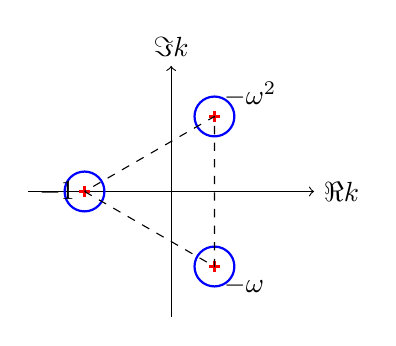
\begin{tikzpicture}[scale=1.1]
  \draw[->] (-1.65,0) -- (1.65,0) node[right] {$\Re k$};
  \draw[->] (0,-1.45) -- (0,1.45) node[above] {$\Im k$};
  \coordinate (a0) at (-1,0);
  \coordinate (a1) at (0.5,-0.866);
  \coordinate (a2) at (0.5,0.866);
  \draw[blue,thick] (a0) circle (0.23);
  \draw[blue,thick] (a1) circle (0.23);
  \draw[blue,thick] (a2) circle (0.23);
  \draw[red,very thick] (-1,-0.06) -- (-1,0.06);
  \draw[red,very thick] (-1.06,0) -- (-0.94,0);
  \draw[red,very thick] (0.5,-0.926) -- (0.5,-0.806);
  \draw[red,very thick] (0.44,-0.866) -- (0.56,-0.866);
  \draw[red,very thick] (0.5,0.806) -- (0.5,0.926);
  \draw[red,very thick] (0.44,0.866) -- (0.56,0.866);
  \node[left] at (a0) {$-1$};
  \node[below right] at (a1) {$-\omega$};
  \node[above right] at (a2) {$-\omega^2$};
  \draw[dashed] (a0) -- (a1) -- (a2) -- cycle;
\end{tikzpicture}
\caption{The cyclic cubic family has three exceptional points forming an
equilateral triangle.  Under $w=k^3+1$, each small meridian maps to a
positive meridian around $0$ in the $w$-plane.}
\label{fig:cyclic-three}
\end{figure}

The eigenvalue equation is
\[
  E^3=w,\qquad w=k^3+1.
\]
Therefore the spectral configuration map factors as
\[
  X\xrightarrow{\;w=k^3+1\;}\bbC^*
  \xrightarrow{\;w\mapsto\{w^{1/3},\omega w^{1/3},\omega^2w^{1/3}\}\;}
  \UConf_3(\bbC).
\]
This factorisation makes the global braid monodromy explicit.

\begin{proposition}[Global braid monodromy of the cyclic cubic family]
Let $g_0,g_1,g_2$ be positive meridians around
$-1,-\omega,-\omega^2$, based at a common point and ordered by any certified
meridian graph.  Under the map $w=k^3+1$, each $g_j$ has winding number one
around $0\in\bbC^*$.  Consequently each generator maps to the same local
cubic braid
\[
  b=\sigma_1\sigma_2\in B_3
\]
up to the simultaneous conjugacy determined by the base paths.  The large
positive circle at infinity maps to
\[
  b^3=(\sigma_1\sigma_2)^3,
\]
the full twist in $B_3$.
\end{proposition}

\begin{proof}
At each zero $a_j$ of $k^3+1$, the derivative $3a_j^2$ is nonzero, so a
small positive meridian around $a_j$ maps to a positive meridian around
$0$ in the $w$-plane.  For $E^3=w$, one positive circuit of $w$ around zero
sends the three local branches cyclically.  With Convention~\ref{conv:upper-half-plane}
(equivalently, the standard local braid convention), this is represented by
$\sigma_1\sigma_2$.  For a large circle
$k=Re^{\ii t}$, one has $w=k^3+1=R^3e^{3\ii t}+1$, so for large $R$ the
image winds three times around zero.  Hence the braid at infinity is the
third power of the local cubic braid.
\end{proof}

\begin{proposition}[Image of the cyclic cubic monodromy]\label{prop:cyclic-image}
For the cyclic cubic family, the braid-monodromy representation factors as
\[
  \pi_1\bigl(\bbC\setminus\{-1,-\omega,-\omega^2\}\bigr)
  \longrightarrow \pi_1(\bbC^*)\cong\bbZ
  \longrightarrow B_3,
\]
where the last map sends \(1\) to \(b=\sigma_1\sigma_2\).  Hence
\[
  \operatorname{Im}\beta_{H_3}=\langle \sigma_1\sigma_2\rangle\cong\bbZ.
\]
The induced permutation monodromy has image the cyclic group \(\bbZ/3\bbZ\).
\end{proposition}

\begin{proof}
The factorisation through \(w=k^3+1\) was established above.  Each finite
meridian has winding number one in \(\bbC^*\), and the cubic-root spectral
cover sends one positive winding to \(b=\sigma_1\sigma_2\).  The element
\(\sigma_1\sigma_2\) has infinite order in \(B_3\), since its cube is the
nontrivial central full twist.  Its image in the symmetric group is the
three-cycle \((123)\), which has order three.
\end{proof}

\begin{remark}[Factorisation versus generic monodromy]
This example is global but not maximally noncommutative: all finite
meridians have the same image in the cyclic subgroup generated by
\(\sigma_1\sigma_2\).  Generic perturbations of the matrix family may break
this factorisation while the graph certificate still applies without
modification.
\end{remark}

\subsection{Certified radius on a meridian graph}

Let $G\subset X$ be any compact meridian graph.  The exact discriminant
margin is
\[
  M_G=27\inf_{k\in G}\abs{k^3+1}^2.
\]
If only samples are available, the certified margin is
\[
  M_G^{\rm cert}=\widehat M_G-\cG_{\cS}(R_*)L_Gh_G.
\]
Because $H_3(k)$ is trace-zero, trace-zero perturbations may use the exact
constant
\[
  \cG_{\tr=0,3}(R_*)=162R_*^5.
\]
If no trace constraint is imposed on the perturbation, one must instead use
an unstructured cubic constant.

For the simple norm bound, note that each row and each column of \(H_3(k)\)
has absolute row or column sum at most \(\abs{k}+1\).  Thus
\[
  \norm{H_3(k)}_1=\norm{H_3(k)}_\infty\le \abs{k}+1,
  \qquad
  \norm{H_3(k)}_2\le
  \sqrt{\norm{H_3(k)}_1\norm{H_3(k)}_\infty}
  \le \abs{k}+1,
\]
by the standard interpolation inequality.  Hence one can take
\[
  R_* > 1+\sup_{k\in G}\abs{k}.
\]
A trace-zero perturbation $\wt H_3:G\to\{A:\tr A=0\}$ is certified to have
the same meridian braids whenever
\[
  \sup_{k\in G}\norm{\wt H_3(k)-H_3(k)}_2
  <
  \frac{M_G^{\rm cert}}{2\cdot 162R_*^5}.
\]

\begin{example}[Three equal circular meridians]
Let $G$ be formed by three small circles
\[
  k=a_j+re^{\ii t},\qquad 0\le t\le2\pi,
\]
joined to a basepoint by arcs staying outside the disks.  On each small
circle,
\[
  k^3+1=3a_j^2re^{\ii t}+O(r^2),
\]
and hence
\[
  \abs{\Delta(k)}=27\abs{k^3+1}^2
  =243r^2+O(r^3).
\]
Thus the certified radius near a small meridian scales like $r^2/R_*^5$ for
operator-norm discriminant certificates.  The braid is nontrivial for every
$r>0$, but the radius collapses quadratically as the meridian approaches the
exceptional point.
\end{example}

%% ===================================================================

\section{Local models and interpretation}\label{sec:local-models}
%% ===================================================================

The two cubic arrangements above are the main examples.  This final section
records, in compressed form, how the same graph certificate interfaces with
standard local braid-monodromy models.

\begin{remark}[Cusp of the versal cubic]\label{rem:cusp}
For the depressed cubic
\[
  P_{u,v}(E)=E^3+uE+v,
  \qquad
  A(u,v)=\begin{pmatrix}0&0&-v\\1&0&-u\\0&1&0\end{pmatrix},
\]
the discriminant is \(\Delta(u,v)=-4u^3-27v^2\).  The cusp
\(4u^3+27v^2=0\) is parametrised by \(u=-3t^2\), \(v=2t^3\).  Projecting
to the \(u\)-line, the two branch values in the \(v\)-fibre are
\[
  v_\pm(u)=\pm \frac{2}{3\sqrt3}(-u)^{3/2}.
\]
When \(u\) winds once around zero, the relative vector
\(v_+(u)-v_-(u)\) rotates through angle \(3\pi\), so the discriminant braid
is \(\tau^3\in B_2\).  This is the classical braid monodromy of the plane
cusp \cite{BrieskornKnoerrer1986,MoishezonTeicher1988}.  Any compact graph in
the complement of the cusp also carries the finite-matrix
discriminant-margin certificate of Theorem~\ref{thm:graph-stab}.
The one-parameter companion cubic \(E^3-3E-k\) is the slice \(u=-3\),
\(v=-k\), where the cusp has split into the two simple branch values
\(k=\pm2\).
\end{remark}

\begin{proposition}[A quartic $A_3$ arrangement with certified radius]
\label{prop:A3-quartic}
For $Q_k(E)=E^4-4E-k$, the derivative $4(E^3-1)$ has critical points
$1,\omega,\omega^2$ with branch values $k_j=-3\omega^j$ ($j=0,1,2$), and
\[
  \Disc(Q_k)=-256(k^3+27).
\]
The polynomial $E^4-4E$ is the standard $A_3$ Morsification
\cite{BrieskornKnoerrer1986}.  In a distinguished $A_3$ Lefschetz basis
the local monodromies at the three branch values are the adjacent half-twists
\[
  \beta(g_1)=\sigma_1,\quad\beta(g_2)=\sigma_2,\quad\beta(g_3)=\sigma_3\in B_4,
\]
forming the $A_3$ Dynkin chain $\sigma_1\text{---}\sigma_2\text{---}\sigma_3$.
The braid at infinity is $\beta(g_\infty)=(\sigma_1\sigma_2\sigma_3)^{-1}$.

For the meridian $k=-3+\rho e^{\ii t}$ around the branch value $k_0=-3$,
the discriminant margin satisfies
\[
  M_\rho=256\min_{|k+3|=\rho}|k^3+27|=256\cdot\min_{|w|=\rho}|w^3-9w^2+27w|
  \approx256\cdot27\rho\quad(\rho\to0).
\]
The companion matrix of $Q_k$ is traceless (its diagonal is zero), so the
traceless $n=4$ discriminant Lipschitz estimate applies.  Using the
unconditional matrix-gradient bound
\(G_4^{\tr=0}(R)\le(60416/3)R^{11}\), the certified perturbation radius is
\[
  \varepsilon_\rho^{\nabla}
  =\frac{M_\rho}{2(60416/3)R_\rho^{11}},
\]
where $R_\rho=\sup_{|k+3|\le\rho}\|A_k\|_2$.
The reduced Pick recursion in Lemma~\ref{lem:reduced-pick-recursion} and the
boundary certificates in Proposition~\ref{prop:reduced-boundary-certificates}
improve this to
\[
  \varepsilon_\rho^{\rm sharp}
  =\frac{M_\rho}{6144R_\rho^{11}},
\]
a factor \(60416/(3\cdot3072)\) over the unconditional matrix-gradient radius.
\end{proposition}

\begin{remark}[Braid at infinity and van Kampen consistency]
For a punctured plane, compactification to the Riemann sphere adds a
meridian \(g_\infty\) satisfying
\[
  g_1\cdots g_m g_\infty=1.
\]
The induced braid representation sends this relation to the identity.  For
the non-abelian cubic one obtains
\(\beta(g_\infty)=(\sigma_1\sigma_2)^{-1}\), in agreement with the
large-parameter asymptotics \(E^3\sim k\).  The graph certificate keeps this
braid at infinity and the finite meridian braids fixed under the same
operator-norm perturbation bound.
\end{remark}

\begin{proposition}[Simple branch values and certified half-twists]\label{prop:PL-half-twist}
Let \(H(k)\) be analytic near \(k=a\).  Suppose that \(H(a)\) has exactly
one repeated eigenvalue of algebraic multiplicity two, with a single Jordan
block on that two-dimensional generalized eigenspace, and all other
eigenvalues are simple and separated.  Then a sufficiently small positive
meridian about \(a\) has spectral braid equal to a simple half-twist, up to
projection and orientation convention.  If the meridian has a certified
positive discriminant margin, this half-twist is stable under all
perturbations inside the corresponding graph radius.
\end{proposition}

\begin{proof}
Weierstrass preparation and the local two-level normal form reduce the
colliding pair to \(E^2=s\) after analytic changes of coordinates; the
remaining eigenvalues stay separated.  A circuit around \(s=0\) exchanges
the two local roots by one half-twist.  The stability statement is exactly
Theorem~\ref{thm:graph-stab} on the small meridian graph.
\end{proof}

\begin{remark}[Interpretation]
For non-Hermitian matrix models, the eigenvalue braid is a topological
charge attached to an exceptional-point arrangement.  The certificate above
turns that charge into a finite statement: on the selected graph, every
listed meridian braid, product relation, and braid at infinity is unchanged
below a computable operator-norm threshold.  The construction is close in
spirit to Picard--Lefschetz and Zariski--van Kampen braid monodromy, but its
input and output are spectral: sampled matrices, braid words, a mesh
correction, and a perturbation radius.
\end{remark}

\begin{remark}[Limitations and further directions]
The companion cubic is surjective onto \(B_3\) but not faithful: its kernel
is the normal closure of the Artin relation.  A sharper example would be a
finite matrix family whose spectral braid monodromy embeds a parameter-domain
group into an Artin group.  On the quantitative side, the main missing
ingredient beyond cubics is a supply of sharp structured
discriminant constants.  The coefficient-box bound of
Proposition~\ref{prop:general-box-Gn} works in every degree, but it becomes
conservative quickly as the resultant degree and the norm scale grow.  A
hybrid implementation should use the polynomial discriminant certificate near
exceptional points and the Bauer--Fike gap certificate on well-conditioned
parts of the graph.  The two-parameter Brillouin torus extension is
developed in Section~\ref{sec:torus}.
\end{remark}


%% ===================================================================
\section{Two-parameter braid monodromy on the Brillouin torus}
\label{sec:torus}
%% ===================================================================

The graph certificate of Section~\ref{sec:graph} is
dimension-free: it uses only a pointwise discriminant Lipschitz estimate and
homotopy invariance into configuration space, so it applies to any compact
parameter space.  This section specialises to the two-dimensional Brillouin
torus \(\bbT^2=S^1\times S^1\), which is the natural parameter space for
two-band non-Hermitian lattice models.  The main content is a precise
identification of the discriminant locus, two versions of the stability
theorem, and an explicit example.

\subsection{Discriminant locus on \(\bbT^2\)}

Write \(z_j=e^{ik_j}\) and let \(H(k_1,k_2)\) be a finite-Fourier analytic
matrix family on \(\bbT^2\).  The discriminant
\[
  \Delta(k_1,k_2)=\Disc(H(k_1,k_2))
\]
is a complex-valued real-analytic function on \(\bbT^2\).  Two cases arise.

\emph{Generic complex case.}
For a general non-Hermitian family, \(\Delta:\bbT^2\to\bbC\) is
complex-valued.  The vanishing set
\(C=\{(k_1,k_2):\Delta(k_1,k_2)=0\}\)
imposes two real equations on the real two-dimensional manifold \(\bbT^2\),
so generically \(C\) is a \emph{finite set of isolated points}.  On the
complexified parameter torus \((\bbC^*)^2\), the zero locus \(\cC_\bbC\)
is a complex algebraic curve; its intersection with the real torus
\(|z_1|=|z_2|=1\) is generically finite.

\emph{Real-discriminant case.}
If \(\Delta\) is real-valued on \(\bbT^2\)---for example, when the matrix
family has a reality symmetry making eigenvalues come in conjugate pairs, or
when a scalar factor forces the discriminant to be real---then \(\Delta=0\)
is a single real equation and \(C\subset\bbT^2\) is generically an embedded
real-analytic curve.  Each connected component of \(C\) is a circle with a
primitive homology class \((p,q)\in H_1(\bbT^2;\bbZ)\cong\bbZ^2\),
\(\gcd(p,q)=1\), or a null-homologous oval.

For a traceless \(n=3\) family with \(\Delta=-4p^3-27q^2\), where
\(p=-\frac12\operatorname{tr}(H^2)\) and \(q=-\det H\) are Laurent
polynomials of bidegree \(\le(2d_1,2d_2)\) and \((3d_1,3d_2)\) respectively,
the discriminant has bidegree at most \((6d_1,6d_2)\).  In the
real-discriminant setting this bounds the topological complexity of \(C\) via
Harnack-type estimates.

\subsection{Fundamental groups}

The relevant fundamental group depends on the type of locus.

\emph{Finite-point locus (\(m\) isolated points).}
\[
  \pi_1(\bbT^2\setminus C)
  \;\cong\;
  \langle a,b,\mu_1,\dots,\mu_m\mid [a,b]\,\mu_1\cdots\mu_m=1\rangle,
\]
where \(a,b\) are the two standard torus generators and each \(\mu_j\) is a
small meridian around the \(j\)-th exceptional point.  After eliminating one
generator this is the free group \(F_{m+1}\).  The two ambient torus cycles
\(a,b\) appear alongside the exceptional-point meridians, carrying additional
braid monodromy absent from the one-parameter punctured-plane setting.

\emph{Embedded curve locus (one component \((p,q)\)-curve).}
If \(C\) is a single embedded essential \((p,q)\)-curve, then
\(\bbT^2\setminus C\) is an open annulus and
\(\pi_1(\bbT^2\setminus C)\cong\bbZ\).

\emph{Zariski--van Kampen presentation.}
In general, project \(\pi:\bbT^2\to S^1\) by \(\pi(k_1,k_2)=k_1\).
Over a regular value the fiber is \(S^1\) punctured at \(d\) points of
\(C\cap\pi^{-1}(k_1)\), giving fiber group \(\pi_1\cong F_d\).  The
monodromy of these punctures as \(k_1\) traverses the finitely many critical
values of \(\pi|_C\) supplies the remaining relations:
\[
  \pi_1(\bbT^2\setminus C)\;=\;
  \bigl\langle\,\pi_1(F_{k_1^0}),\,\gamma_1,\dots,\gamma_\ell,\,\eta\;\big|\;
  \gamma_j x\gamma_j^{-1}=\rho_j(x),\;\eta x\eta^{-1}=\rho_\infty(x),\;
  \gamma_1\cdots\gamma_\ell=\eta\,\bigr\rangle,
\]
where \(\rho_j\) is the fiber braid monodromy at the \(j\)-th critical value
and \(\eta\) records the total monodromy of the base \(S^1\).

\subsection{Stability theorems}

Two distinct stability statements arise, according to whether \(M_{\bbT^2}>0\).

\begin{theorem}[Full-torus stability]\label{thm:torus-full}
Let \(H:\bbT^2\to\cS\subset M_n(\bbC)\) be continuous, with
\(\sup_{\bbT^2}\|H(k)\|_2\le R\) and
\[
  M_{\bbT^2}:=\inf_{k\in\bbT^2}|\Delta(k)|>0.
\]
Choose \(R_*>R\) and let \(\cG_\cS(R_*)\) be an admissible discriminant
Lipschitz constant on \(\cS\cap\{\|A\|_2\le R_*\}\).  If
\[
  \sup_{\bbT^2}\|\widetilde H(k)-H(k)\|_2
  <
  \min\!\left\{R_*-R,\;\frac{M_{\bbT^2}}{2\cG_\cS(R_*)}\right\},
\]
then \(H_t=(1-t)H+t\widetilde H\) has simple spectrum on all of \(\bbT^2\)
for every \(t\in[0,1]\), and the spectral braid representations
\(\phi_H,\phi_{\widetilde H}:\pi_1(\bbT^2)\to B_n\) are equal up to
simultaneous conjugacy.
\end{theorem}

\begin{proof}
The Lipschitz estimate gives, pointwise in \(k\),
\[
  |\Delta(H_t(k))-\Delta(H(k))|
  \le \cG_\cS(R_*)\sup\|\widetilde H-H\|_2
  < M_{\bbT^2}/2,
\]
so \(|\Delta(H_t(k))|\ge M_{\bbT^2}/2>0\) for all \(t,k\).  The
map \((t,k)\mapsto\Lambda_{H_t}(k)\) is therefore a homotopy of
\(\bbT^2\to\UConf_n(\bbC)\).  Homotopic maps induce equal representations
on \(\pi_1\), up to the basepoint-identification conjugacy.
\end{proof}

\begin{remark}
\(M_{\bbT^2}>0\) is equivalent to \(C=\varnothing\).  When \(C\neq\varnothing\),
\(M_{\bbT^2}=0\) and Theorem~\ref{thm:torus-full} does not apply.  The
correct object is then a positive margin on a compact
\(K\subset\bbT^2\setminus C\).
\end{remark}

\begin{theorem}[Torus graph stability]\label{thm:torus-graph}
Let \(K\subset\bbT^2\setminus C\) be a compact subset whose inclusion
induces a surjection \(\pi_1(K)\twoheadrightarrow\pi_1(\bbT^2\setminus C)\),
for example a deformation retract or a carrying graph.  Assume
\(\sup_K\|H(k)\|_2\le R\) and \(M_K:=\inf_K|\Delta(k)|>0\).  If
\[
  \sup_K\|\widetilde H(k)-H(k)\|_2
  <
  \min\!\left\{R_*-R,\;\frac{M_K}{2\cG_\cS(R_*)}\right\},
\]
then the induced representations
\(\phi_H,\phi_{\widetilde H}:\pi_1(K)\to B_n\)
are equal up to simultaneous conjugacy; and if \(K\simeq\bbT^2\setminus C\),
then so are the full complement representations.
\end{theorem}

\begin{proof}
This is exactly Theorem~\ref{thm:graph-stab} with \(\cP=\bbT^2\).  The
proof is pointwise in matrix space and does not depend on the dimension of
the parameter space.
\end{proof}

For traceless \(3\times3\) families, both theorems use
\(\cG_{\tr=0,3}(R_*)=162R_*^5\) from Section~\ref{sec:tr0constant}.

\subsection{Equivalence relation for two-parameter braid monodromy}

For a one-parameter loop, the invariant is a conjugacy class in \(B_n\).
For the two-parameter representation
\(\phi_H:\pi_1(\bbT^2\setminus C,p_0)\to B_n\),
the correct equivalence is \emph{simultaneous conjugacy}: two representations
\(\phi,\widetilde\phi\) are equivalent if there exists \(b\in B_n\) with
\[
  \widetilde\phi(\gamma)=b\,\phi(\gamma)\,b^{-1}
  \qquad\text{for all }\gamma\in\pi_1(\bbT^2\setminus C,p_0).
\]
If the basepoint or generating system changes, one additionally precomposes
with the induced automorphism of \(\pi_1(\bbT^2\setminus C)\).  This is
strictly stronger than checking individual braid words: the representation
records non-abelian relations between the two ambient torus cycles, the
exceptional-point meridians, and any torus relation they satisfy.

\subsection{Two-parameter Hatano--Nelson example}

Let \(M=J_\omega=\diag(1,\omega,\omega^2)\), \(\omega=e^{2\pi i/3}\), and
define
\[
  H(k_1,k_2)=f(k_1,k_2)I+g(k_1,k_2)M,
\]
where \(f,g\) are Laurent polynomials.  Since eigenvalue differences
scale by \(g\), we have
\[
  \Delta(k_1,k_2)=\Disc(M)\cdot g(k_1,k_2)^6=-27\,g(k_1,k_2)^6.
\]

\emph{Example A (real \(\Delta\), embedded curve \(C\)).}
Take
\[
  g(k_1,k_2)=m+t_1\cos k_1+t_2\cos k_2,\qquad m,t_1,t_2\in\bbR.
\]
Then \(\Delta\in\bbR\) on \(\bbT^2\) and
\(C=\{m+t_1\cos k_1+t_2\cos k_2=0\}\).
If \(|m|>|t_1|+|t_2|\) then \(C=\varnothing\) and \(M_{\bbT^2}=27\inf|g|^6>0\);
Theorem~\ref{thm:torus-full} gives an explicit radius with
\(\cG_{\tr=0,3}(R_*)=162R_*^5\).
If \(|m|<|t_1|+|t_2|\) then \(C\) is a non-empty embedded curve;
\(\pi_1(\bbT^2\setminus C)\) is a free group, and the graph certificate
of Theorem~\ref{thm:torus-graph} applies on any compact carrying subgraph.

\emph{Example B (non-real \(\Delta\), finite \(C\)).}
Take
\[
  g(k_1,k_2)=ae^{\ii k_1}+be^{-\ii k_1}+ce^{\ii k_2}-\gamma,\qquad a\ne b.
\]
Then \(\Delta=-27g^6\) is complex-valued.  Its zero set
\(C=\{g=0\}\subset\bbT^2\) is generically a pair of isolated exceptional
points.  The group \(\pi_1(\bbT^2\setminus C)\cong F_3\) has generators
\(a,b,\mu_1,\mu_2\) with relation \([a,b]\mu_1\mu_2=1\).
Since all eigenvalues of \(H=gM\) rotate rigidly together, every generator
maps into the centre \(Z(B_3)\); the image is a cyclic group.
The no-puncture case is computed in
Proposition~\ref{prop:T2-no-puncture}; the diagnostic non-generic scalar
family in Proposition~\ref{prop:T2-degenerate-three-zero} records what goes
wrong if the discriminant has an additional non-transverse zero.

\begin{proposition}[Full-torus monodromy, no exceptional points]
\label{prop:T2-no-puncture}
Let $M=\diag(1,\omega,\omega^2)$, $\omega=e^{2\pi\ii/3}$,
$H(k_1,k_2)=g(k_1,k_2)M$ with
\[
  g(k_1,k_2)=e^{\ii k_1}+0.3e^{-\ii k_1}+0.5e^{\ii k_2}.
\]
Since $|e^{\ii k_1}+0.3e^{-\ii k_1}|^2=1.09+0.6\cos(2k_1)\ge0.49$, we
have $|e^{\ii k_1}+0.3e^{-\ii k_1}|\ge0.7>0.5$ for all $k_1$, so $g$
has no zeros on $\bbT^2$ and $M_{\bbT^2}>0$.

The spectral braid monodromy $\phi:\pi_1(\bbT^2)\cong\bbZ^2\to B_3$ is
computed from the winding numbers of $g$ along the two standard cycles.
Along $k_1:0\to2\pi$ with $k_2=0$ fixed, $g=e^{\ii k_1}+0.3e^{-\ii k_1}+0.5$
has winding number $w_1=1$ around $0$.  Along $k_2:0\to2\pi$ with $k_1=0$,
$g=1.3+0.5e^{\ii k_2}$ satisfies $|g|\ge0.8>0$, so $w_2=0$.
A winding-number-$w$ loop of $g$ rotates all three eigenvalues
$g,g\omega,g\omega^2$ rigidly by $2\pi w$, corresponding to the $w$-th power
of the positive full twist $\Omega=(\sigma_1\sigma_2)^3\in Z(B_3)$.
Therefore
\[
  \phi(\alpha_1)=(\sigma_1\sigma_2)^3,\qquad\phi(\alpha_2)=1,
  \qquad\phi(m,n)=\bigl((\sigma_1\sigma_2)^3\bigr)^m.
\]
The image is the cyclic subgroup
\(\langle(\sigma_1\sigma_2)^3\rangle\cong\bbZ\) of \(Z(B_3)\).
Theorem~\ref{thm:torus-full} applies with
$\cG_{\tr=0,3}(R_*)=162R_*^5$.
\end{proposition}

\begin{proposition}[Diagnostic non-generic torus scalar family]
\label{prop:T2-degenerate-three-zero}
Keep $H=gM$ with
\[
  g(k_1,k_2)=e^{\ii k_1}+0.3e^{-\ii k_1}+0.5e^{\ii k_2}-0.8.
\]
The equation $g=0$ on $\bbT^2$ has two transverse zeros, located at
\begin{align*}
  p_1 &= \bigl(\arccos\tfrac{11}{15},\;\pi+\arccos\tfrac{23}{75}\bigr)
        \approx(0.7476,\,4.4007),\\
  p_2 &= \bigl(2\pi-\arccos\tfrac{11}{15},\;\pi-\arccos\tfrac{23}{75}\bigr)
        \approx(5.5356,\,1.8825),
\end{align*}
with Jacobians
\[
  J(p_1)=-\tfrac{8\sqrt{26}}{375}<0,\qquad J(p_2)=+\tfrac{8\sqrt{26}}{375}>0.
\]
It also has a third, non-transverse zero at
\[
  p_0=(0,\pi).
\]
Thus the correct discriminant complement is
\(\bbT^2\setminus\{p_0,p_1,p_2\}\), not a two-puncture torus.  This example is
therefore recorded only as a diagnostic non-generic scalar family; it is not
used as a two-puncture monodromy computation.
\end{proposition}

\begin{proof}
Write $c=\cos k_1$, $s=\sin k_1$, $C=\cos k_2$, $S=\sin k_2$.  The
condition $g=0$ is equivalent to the real system
\[
  1.3c+0.5C=0.8,\qquad 0.7s+0.5S=0.
\]
The second equation gives $S=-1.4s$; substituting $C=(0.8-1.3c)/0.5$ into
$C^2+S^2=1$ and expanding with $s^2=1-c^2$ yields
\[
  15c^2-26c+11=(15c-11)(c-1)=0,
\]
so $c\in\{1,\,11/15\}$.

\emph{Case $c=1$} ($k_1=0$, $S=0$, $C=-1$, $k_2=\pi$).
The Jacobian of the real map $(k_1,k_2)\mapsto(\operatorname{Re}g,\operatorname{Im}g)$ is
\[
  J(k_1,k_2)=-0.65\sin k_1\cos k_2+0.35\sin k_2\cos k_1.
\]
At $(0,\pi)$: $J=0$.  A local expansion gives
$g(\epsilon,\pi+\delta)\approx(-0.65\epsilon^2+0.25\delta^2)+i(0.7\epsilon-0.5\delta)$,
so on the circle $(\epsilon,\delta)=r(\cos\theta,\sin\theta)$ the
image of $g$ stays near the imaginary axis to leading order and does not
wind around the origin; the local degree of $g$ at $(0,\pi)$ is zero.
This zero may carry trivial local winding, but it is still part of the
discriminant locus and cannot be deleted from the domain.

\emph{Case $c=11/15$}.  Then $s=\pm2\sqrt{26}/15$,
$C=-23/75$, $S=\mp14\sqrt{26}/75$.  (One checks $C^2+S^2=(529+196\cdot26)/75^2=1$.)
The two solutions are $p_1$ (sign $+$) and $p_2$ (sign $-$), with coordinates
as stated.  The Jacobian formula gives
\begin{align*}
  J(p_{1,2})
  &=-0.65\cdot\bigl(\pm\tfrac{2\sqrt{26}}{15}\bigr)\cdot\bigl(-\tfrac{23}{75}\bigr)
   +0.35\cdot\bigl(\mp\tfrac{14\sqrt{26}}{75}\bigr)\cdot\tfrac{11}{15}\\
  &=\frac{\sqrt{26}}{22500}\bigl(\pm598\mp1078\bigr)
   =\mp\frac{8\sqrt{26}}{375},
\end{align*}
confirming $\sgn J(p_1)=-1$ and $\sgn J(p_2)=+1$.

This completes the stated diagnostic calculation.
\end{proof}

\appendix

\section{Takenaka--Malmquist entries for the quartic gradient}\label{app:tm-entries}
Let \(\ell_i=\lambda_i\) and \(d_i=(1-|\lambda_i|^2)^{1/2}\).  For the
rank-one defect model \(S_B\), the upper triangular entries of
\[
  A_B=c_1S_B+c_2S_B^2+c_3S_B^3
\]
are
\[
\begin{aligned}
(A_B)_{11}&=\ell_1(c_1+c_2\ell_1+c_3\ell_1^2),\\
(A_B)_{12}&=d_1d_2\{c_1+c_2(\ell_1+\ell_2)
  +c_3(\ell_1^2+\ell_1\ell_2+\ell_2^2)\},\\
(A_B)_{13}&=-d_1d_3\{c_1\ell_2-c_2d_2^2+c_2\ell_1\ell_2+c_2\ell_2\ell_3\\
&\hspace{2.7cm}
-c_3d_2^2(\ell_1+\ell_2+\ell_3)
+c_3\ell_1^2\ell_2+c_3\ell_1\ell_2\ell_3+c_3\ell_2\ell_3^2\},\\
(A_B)_{14}&=d_1d_4\{c_1\ell_2\ell_3-c_2d_2^2\ell_3-c_2d_3^2\ell_2
+c_2\ell_1\ell_2\ell_3+c_2\ell_2\ell_3\ell_4\\
&\hspace{2.7cm}
+c_3d_2^2d_3^2-c_3d_2^2(\ell_1\ell_3+\ell_2\ell_3+\ell_3\ell_4)\\
&\hspace{2.7cm}
-c_3d_3^2(\ell_1\ell_2+\ell_2\ell_3+\ell_2\ell_4)
+c_3\ell_1^2\ell_2\ell_3\\
&\hspace{2.7cm}
+c_3\ell_1\ell_2\ell_3\ell_4+c_3\ell_2\ell_3\ell_4^2\},\\
(A_B)_{22}&=\ell_2(c_1+c_2\ell_2+c_3\ell_2^2),\\
(A_B)_{23}&=d_2d_3\{c_1+c_2(\ell_2+\ell_3)
  +c_3(\ell_2^2+\ell_2\ell_3+\ell_3^2)\},\\
(A_B)_{24}&=-d_2d_4\{c_1\ell_3-c_2d_3^2+c_2\ell_2\ell_3+c_2\ell_3\ell_4\\
&\hspace{2.7cm}
-c_3d_3^2(\ell_2+\ell_3+\ell_4)
+c_3\ell_2^2\ell_3+c_3\ell_2\ell_3\ell_4+c_3\ell_3\ell_4^2\},\\
(A_B)_{33}&=\ell_3(c_1+c_2\ell_3+c_3\ell_3^2),\\
(A_B)_{34}&=d_3d_4\{c_1+c_2(\ell_3+\ell_4)
  +c_3(\ell_3^2+\ell_3\ell_4+\ell_4^2)\},\\
(A_B)_{44}&=\ell_4(c_1+c_2\ell_4+c_3\ell_4^2).
\end{aligned}
\]

\section{Pick certificate data for the quartic Blaschke model}
\label{app:pick-certificate}
This appendix gives the finite calculation associated with
Remark~\ref{conj:pick-blaschke-certificate}.  The centred constraint is imposed by
\[
  \lambda_4=-(\lambda_1+\lambda_2+\lambda_3).
\]
Let \(q_i=q_\lambda(\lambda_i)\), where
\[
  q_\lambda(z)=768^{-1}(c_1z+c_2z^2+c_3z^3).
\]
The four values \(q_i\) are homogeneous polynomials of degree \(11\) divided
by \(192\).
For example,
\[
  q_1=\frac{\lambda_1}{192}\,Q_1(\lambda_1,\lambda_2,\lambda_3),
\]
where \(Q_1\) is a degree-ten integer polynomial.  The other \(q_i\) are
obtained by permuting the centred roots.

The reduced data used in the non-normal certificate are
\[
  r_i=\frac{q_i}{\lambda_i}
  =768^{-1}(c_1+c_2\lambda_i+c_3\lambda_i^2),
\]
with the limiting value understood when \(\lambda_i=0\).  The reduced Pick
matrix is
\[
  \Pi^{\rm red}_\lambda=\left[
  \frac{1-r_i\overline{r_j}}{1-\lambda_i\overline{\lambda_j}}
  \right]_{i,j=1}^4.
\]
The verification is carried out on principal submatrices of
\(\Pi^{\rm red}_\lambda\).  For a fixed ordering \(\alpha\) and a principal
index set \(I\), use the Schur complement recursion
\[
  \Pi^{(1)}=\Pi,\qquad
  \Pi^{(m+1)}=\Pi^{(m)}_{22}
  -\Pi^{(m)}_{21}\bigl(\Pi^{(m)}_{11}\bigr)^{-1}\Pi^{(m)}_{12},
\]
with the rows and columns ordered by \(\alpha\).  Clearing the positive
denominators
\[
  D_m=\prod_{i,j\le m}(1-\lambda_i\overline{\lambda_j})
  \prod_{p<q}|\lambda_p-\lambda_q|^{2e_m}
\]
gives scalar real polynomials \(R_{I,\alpha,m}\) after the substitutions
\[
  \lambda_j=x_j+\ii y_j,\qquad
  \overline{\lambda_j}=x_j-\ii y_j,\qquad
  x_4+\ii y_4=-(\lambda_1+\lambda_2+\lambda_3).
\]
Thus
\[
  R_{I,\alpha,m}\in
  \bbZ[x_1,y_1,x_2,y_2,x_3,y_3].
\]
The sign condition for the reduced Pick matrix is exactly
\[
  R_{I,\alpha,m}\ge0
\]
on the semialgebraic chamber
\[
  x_j^2+y_j^2\le1,\qquad
  (x_i-x_j)^2+(y_i-y_j)^2>0,\qquad
  |\lambda_{\alpha(1)}|\ge\cdots\ge|\lambda_{\alpha(4)}|.
\]

For the compact Bernstein check, rotate so that \(\lambda_{\alpha(1)}=\rho\)
with \(0\le\rho\le1\), write the remaining two free roots as
\[
  \lambda_{\alpha(2)}=\rho_2 e^{\ii\theta_2},\qquad
  \lambda_{\alpha(3)}=\rho_3 e^{\ii\theta_3},
\]
and set
\[
  X_0=\rho,\quad X_1=\rho_2^2,\quad X_2=\rho_3^2,\quad
  X_3=\cos\theta_2,\quad X_4=\sin\theta_2,\quad
  X_5=\cos\theta_3,\quad X_6=\sin\theta_3 .
\]
The two circle relations \(X_3^2+X_4^2=1\),
\(X_5^2+X_6^2=1\) are eliminated boxwise by the tangent half-angle
substitution on four angular charts.  Each chamber polynomial therefore
becomes a finite list of ordinary real polynomials on boxes \([0,1]^6\).
Bernstein subdivision is valid because every denominator removed above is
strictly positive on the interior of the chamber, and the boundary boxes are
precisely the normal, \(3{+}1\), paired, radial-square, or confluent faces
already certified in the main text.

The exact-arithmetic certificate is therefore a finite table:
for each tuple \((I,\alpha,m,\nu)\), where \(\nu\) indexes the chamber and
angular chart, list the Bernstein degree vector \(d_{I,\alpha,m,\nu}\) and the
minimum Bernstein coefficient
\[
  \beta_{I,\alpha,m,\nu}^{\min}\ge0 .
\]
Strictly positive \(\beta^{\min}\) proves the corresponding box immediately;
zero coefficients are admissible only on one of the already certified boundary
faces.  This is the exact form in which the remaining interior certificate is
finite and machine-checkable.

\begin{remark}[Why the resolved certificate is used]\label{rem:direct-bernstein-size}
The direct five-real-variable Bernstein table is finite but too large to serve
as a useful printed certificate.  Expanding only the \(2\times2\) reduced Pick
minor numerators in the centred variables
\[
  \lambda_1=r_1,\qquad \lambda_2=x_2+\ii y_2,\qquad
  \lambda_3=x_3+\ii y_3,\qquad
  \lambda_4=-(\lambda_1+\lambda_2+\lambda_3)
\]
already gives total degree \(42\).  The six unordered pairs have respectively
\[
\begin{array}{c|cccccc}
\{i,j\}&12&13&14&23&24&34\\ \hline
\#\text{ monomials}&100400&100400&101780&103234&103210&103210 .
\end{array}
\]
Thus the brute-force table is a legitimate finite verification problem, while
the printed proof uses a smaller certificate: the lower-dimensional
Schur-pivot certificate isolates the radial-square degeneration, and
Appendix~\ref{app:gamma-three-hard-corner} resolves the only hard Bernstein
corner by a blow-up.
\end{remark}

\begin{remark}[Finite termination of the certificate]\label{rem:finite-certificate-termination}
The reduction stops at a finite exact-arithmetic problem.  No new analytic or
functional-analytic statement remains after
Proposition~\ref{prop:finite-interior-reduction}: the objects to be checked are
explicitly generated polynomials with rational coefficients on rational boxes.
This article supplies the resolved certificate for the unique hard corner in
Appendix~\ref{app:gamma-three-hard-corner}.  The regular chamber certificates
are listed in the supplementary manifest cited in
Proposition~\ref{prop:interior-machine-certificate}.  Together these finite
exact-arithmetic checks close the non-normal quartic case.
\end{remark}

\begin{lemma}[Bernstein certificate implication]\label{lem:bernstein-certificate-implication}
Let \(P\in\bbQ[t_1,\ldots,t_s]\) and let \(Q=\prod_a q_a\) be a product of
constraint polynomials which are non-negative on a box \(B\subset[0,1]^s\).
Suppose that, after subdivision of \(B\) into finitely many rational boxes
\(B_\nu\), one has an identity
\[
  P=B_\nu^{(0)}+\sum_a q_a M_{a,\nu}
\]
\[
  \text{on }B_\nu,
\]
where \(B_\nu^{(0)}\) and every multiplier \(M_{a,\nu}\) have non-negative
Bernstein coefficients on \(B_\nu\).
Then \(P\ge0\) on \(B\).  If the only zero Bernstein coefficients occur on
faces contained in the union of the certified boundary strata, then \(P>0\) on
the genuinely interior non-confluent part of \(B\).
\end{lemma}

\begin{proof}
The Bernstein basis is a partition of unity by non-negative polynomials on a
box.  Therefore a polynomial with non-negative Bernstein coefficients is
non-negative throughout that box.  Since \(q_a\ge0\) and
\(M_{a,\nu}\ge0\), the displayed identity gives \(P\ge0\) on \(B_\nu\).
The sign of \(P\) on the whole chamber follows after summing over the finite
subdivision.  The strict statement follows because a Bernstein zero can persist
in the interior only if every active basis term carrying that point has zero
coefficient; by the certificate table these zero terms are supported only on
the already certified boundary faces.
\end{proof}

\section{Pair-defect Blaschke certificate}\label{app:pair-defect-blaschke}
The reduced Pick problem is closed on the whole paired locus.  After a common
rotation, write a paired centred spectrum as
\[
  \{1,-1,z,-z\},\qquad |z|\le1.
\]
For the reduced data
\[
  r_i=768^{-1}\bigl(c_1+c_2\lambda_i+c_3\lambda_i^2\bigr)
\]
one obtains
\[
\begin{aligned}
  r(1)=r(-1)&=A(z):=\frac{z^2(1-z^2)^3(5-z^2)}{48},\\
  r(z)=r(-z)&=B(z):=\frac{(1-z^2)^3(1-5z^2)}{48}.
\end{aligned}
\]
The Schur algorithm for the data
\((1,A),(-1,A),(z,B),(-z,B)\) gives
\[
  A,\qquad 0,\qquad -\,\frac{B-A}{1-\overline A B},\qquad 0.
\]
Thus the reduced Pick matrix is positive semidefinite as soon as
\(|A|,|B|\le1\).  For \(|z|\le1\),
\[
  |A|\le \frac{|z|^2|1-z^2|^3|5-z^2|}{48}
  \le \frac{1\cdot 2^3\cdot 6}{48}=1,
\]
and
\[
  |B|\le \frac{|1-z^2|^3|1-5z^2|}{48}
  \le \frac{2^3\cdot 6}{48}=1.
\]
Equality in both estimates can occur only at \(z^2=-1\), namely the square
\(\{1,-1,\ii,-\ii\}\).  Hence the paired-locus reduced Pick certificate is
unconditional.

The adjacent one-defect boundary edge also has a terminating certificate.  On
the centred \(3{+}1\) edge
\[
  \{1,e^{\ii\theta},e^{-\ii\theta},-r\},\qquad
  \cos\theta=\frac{r-1}{2},\qquad 0\le r\le1,
\]
the reduced Schur gaps factor as rational functions of \(r\).  The numerators
are products of powers of \(1-r\) and the following real factors:
\[
\begin{aligned}
p_9&=4r^9-16r^8-15r^7+81r^6+25r^5-91r^4+71r^3+15r^2-165r-165,\\
p_{10}&=4r^{10}-20r^9+r^8+96r^7-56r^6-116r^5+162r^4-56r^3-180r^2-219,\\
p_{18}&=8r^{18}-36r^{17}-126r^{16}+703r^{15}+160r^{14}-3193r^{13}\\
&\quad+2299r^{12}+945r^{11}-9684r^{10}+14733r^9+14163r^8-6135r^7\\
&\quad+24992r^6+21897r^5+1737r^4+24039r^3+37836r^2+36135r+36135 .
\end{aligned}
\]
Sturm's theorem gives no roots in \([0,1]\) for these three polynomials; their
endpoint signs are
\[
  p_9(0),p_9(1)<0,\qquad p_{10}(0),p_{10}(1)<0,\qquad
  p_{18}(0),p_{18}(1)>0 .
\]
The denominator factors have the same Sturm verification and positive endpoint
signs.  Therefore the reduced Pick matrix is positive on this one-defect edge,
with degeneration only at \(r=1\), where it lands on the square.

The first reduced pivot on the full two-angle \(3{+}1\) stratum has a finite
certificate.  Write
\[
  P(z)=(z+r)(z^3-rz^2+u r z-u),\qquad u=e^{\ii\chi},\qquad 0\le r\le1.
\]
The interior node is \(-r\).  Direct substitution in the reduced value
\[
  r(\lambda)=768^{-1}(c_1+c_2\lambda+c_3\lambda^2)
\]
gives
\[
  1-|r(-r)|^2=\frac{M(r,\cos\chi)}{36864},
\]
where \(M\) is a polynomial of bidegree \((18,4)\) after the change
\(\cos\chi=2y-1\).  In the Bernstein basis on
\((r,y)\in[0,1]^2\), all \(95\) coefficients of \(M(r,2y-1)\) are
non-negative, and the only common zero of the certificate is the square
endpoint \((r,y)=(1,1)\).

It remains to control the three unit boundary nodes.  By rotation it suffices
to fix one of them at \(1\).  Let the other two unit nodes be \(x,y\in\partial
\bbD\) and put
\[
  s=x+y,\qquad xy=s/\overline s,\qquad |1+s|\le1 .
\]
The last inequality is exactly the condition that the fourth root
\(-(1+x+y)\) lies in \(\overline\bbD\).  For the selected unit node \(1\), the
same substitution gives
\[
  1-|r(1)|^2
  =\frac{N(a,b)}{36864(a^2+b^2)^4},\qquad s=a+\ii b.
\]
Set \(s=-1+\rho e^{\ii\psi}\) and \(\cos\psi=2y-1\).  Since the denominator is
positive away from the square limit \(s=0\), it suffices to prove
\[
  \mathcal N(\rho,y):=N(-1+\rho(2y-1),\,\rho\sqrt{1-(2y-1)^2})\ge0
\]
on \([0,1]^2\).  The square root is harmless because \(N(a,b)\) is even in
\(b\), so \(\mathcal N\) is an ordinary polynomial.  Its bidegree is
\((28,13)\) and it has \(223\) non-zero monomial terms.  Exact rational
Bernstein expansion on the following dyadic subdivision gives:
\[
\begin{array}{c|c|c}
\rho\text{-interval} & y\text{-interval} & \min\text{ Bernstein coefficient}\\ \hline
\lbrack 0,1/2\rbrack & \lbrack 0,1\rbrack & 32343111/262144\\
\lbrack 1/2,1\rbrack & \lbrack 0,1/2\rbrack & 0\\
\lbrack 1/2,1\rbrack & \lbrack 1/2,1\rbrack & 0 .
\end{array}
\]
Hence \(\mathcal N\ge0\) on the whole square.  The zero coefficients in the
last two boxes occur only on the endpoint faces corresponding to the square
configuration, so the inequality is strict away from that endpoint.  Therefore
\(|r_i|\le1\) for all four nodes on the full \(3{+}1\) stratum.  This proves
the first reduced Schur pivot on that stratum.  Together with the radial
boundary blow-up lemma (Lemma~\ref{lem:radial-boundary-blowup}), the strict
unit-node inequalities away from the square imply the full reduced Pick
certificate on the general two-angle \(3{+}1\) boundary.

There is also a closed two-boundary/two-interior radial edge.  For
\[
  \{1,-1,\ii r,-\ii r\},\qquad 0\le r\le1,
\]
the reduced Schur gaps are
\[
\begin{aligned}
G_1&=\frac{(1-r^2)(r^2+3)(r^6+6r^4+9r^2+16)
(r^{10}+8r^8+18r^6+16r^4+5r^2+48)}{2304},\\
G_2&=1,\qquad G_4=1,
\end{aligned}
\]
and
\[
G_3=
\frac{(1-r^2)^2 (r^2+3)(r^6+6r^4+9r^2+16)
(5r^6+21r^4+39r^2+47)}
     {(5r^{18}+56r^{16}+236r^{14}+520r^{12}+670r^{10}
       +520r^8+236r^6+56r^4+5r^2+2304)^2}
\]
multiplied by the positive factors
\[
 (5r^8+16r^6+18r^4+8r^2+49)
 (r^{10}+8r^8+18r^6+16r^4+5r^2+48).
\]
Thus this radial two-pair edge is positive for \(0\le r<1\) and becomes sharp
only at the square.

For the extremal two-defect Blaschke submodel with ordered spectrum
\(\{1,ir,-ir,-1\}\), \(0\le r\le1\), the Takenaka--Malmquist matrix gives
\[
\sum_{i\le j}|(A_B)_{ij}|
= -16(1+r)(1+r^2)^3(3r^3-13r^2-r-1).
\]
Therefore
\[
3072-\sum_{i\le j}|(A_B)_{ij}|
=16(r-1)h_9(r),
\]
where
\[
 h_9(r)=3r^9-7r^8-12r^7-44r^6-78r^5-114r^4-156r^3-172r^2-189r-191.
\]
Since all coefficients of \(h_9'(r)\) except the first are negative and
\(h_9(1)=-960<0\), Sturm's theorem (or direct monotonicity after one derivative
split) gives \(h_9(r)<0\) on \([0,1]\).  Hence the pair-defect submodel satisfies
\[
\sum_{i\le j}|(A_B)_{ij}|\le3072,
\]
with equality only at \(r=1\).

For the Frobenius check on the pair-defect edge, the same substitution gives
\[
  \|A_B\|_{\mathrm F}^2
  =256(1+r^2)^6(27r^8+30r^6+76r^4+10r^2+1).
\]
Consequently
\[
  1536^2-\|A_B\|_{\mathrm F}^2=256(1-r^2)k_{18}(r),
\]
where
\[
\begin{aligned}
k_{18}(r)={}&27r^{18}+219r^{16}+880r^{14}+2336r^{12}+4542r^{10}\\
&+6830r^8+8392r^6+9048r^4+9199r^2+9215 .
\end{aligned}
\]
Thus the Frobenius certificate is strict on this submodel for \(0\le r<1\)
and becomes sharp only at \(r=1\).

\section{Bernstein--Sturm data for the quartic $(3+1)$ monotonicity}\label{app:bernstein-3plus1}
This appendix lists the Bernstein coefficients in $w=(1+c)/2$ used in the proof that $\partial_c\mathcal B\ge0$.
\begingroup
\scriptsize
\subsection*{$R$}
Degree in $w$: $2$.
\[
\resizebox{\textwidth}{!}{$\begin{aligned}
b_{0}(r)&=\left(r - 1\right) \left(730 r^{9} - 910 r^{8} - 1355 r^{7} - 1963 r^{6} - 63 r^{5} - 711 r^{4} + 823 r^{3} - 377 r^{2} - 135 r - 135\right),\quad b_{0}(0)=135,\quad b_{0}(1)=0,\quad \text{only the displayed endpoint zero}\\
b_{1}(r)&=730 r^{10} - 1725 r^{8} + 620 r^{6} + 1534 r^{4} + 242 r^{2} + 135,\quad b_{1}(0)=135,\quad b_{1}(1)=1536,\quad \text{no zero in }(0,1)\\
b_{2}(r)&=\left(r + 1\right) \left(730 r^{9} + 910 r^{8} - 1355 r^{7} + 1963 r^{6} - 63 r^{5} + 711 r^{4} + 823 r^{3} + 377 r^{2} - 135 r + 135\right),\quad b_{2}(0)=135,\quad b_{2}(1)=8192,\quad \text{no zero in }(0,1)\\
\end{aligned}$}
\]
\subsection*{$-E$}
Degree in $w$: $2$.
\[
\resizebox{\textwidth}{!}{$\begin{aligned}
b_{0}(r)&=- \left(r - 1\right) \left(r + 3\right)^{2} \left(2 r^{2} + r + 1\right) \left(2 r^{5} + 9 r^{4} - 24 r^{3} + 17 r^{2} - 24 r + 36\right),\quad b_{0}(0)=324,\quad b_{0}(1)=0,\quad \text{only the displayed endpoint zero}\\
b_{1}(r)&=- 4 r^{10} - 235 r^{8} - 69 r^{6} - r^{4} + 369 r^{2} + 324,\quad b_{1}(0)=324,\quad b_{1}(1)=384,\quad \text{no zero in }(0,1)\\
b_{2}(r)&=- \left(r - 3\right)^{2} \left(r + 1\right) \left(2 r^{2} - r + 1\right) \left(2 r^{5} - 9 r^{4} - 24 r^{3} - 17 r^{2} - 24 r - 36\right),\quad b_{2}(0)=324,\quad b_{2}(1)=1728,\quad \text{no zero in }(0,1)\\
\end{aligned}$}
\]
\subsection*{$-N$}
Degree in $w$: $3$.
\[
\resizebox{\textwidth}{!}{$\begin{aligned}
b_{0}(r)&=- \left(r - 1\right)^{2} \left(r + 3\right)^{2} \left(2 r^{2} + r + 1\right) \left(68 r^{10} + 30 r^{9} - 1204 r^{8} - 421 r^{7} - 653 r^{6} + 2671 r^{5} + 931 r^{4} + 2905 r^{3} - 4067 r^{2} - 1089 r - 3267\right),\quad b_{0}(0)=29403,\quad b_{0}(1)=0,\quad \text{only the displayed endpoint zero}\\
b_{1}(r)&=- \frac{\left(r - 1\right) \left(408 r^{15} + 1080 r^{14} + 15990 r^{13} - 17634 r^{12} - 63039 r^{11} - 99031 r^{10} - 41407 r^{9} - 48943 r^{8} + 86114 r^{7} + 38610 r^{6} + 17448 r^{5} + 109296 r^{4} + 121557 r^{3} + 227421 r^{2} + 88209 r + 88209\right)}{3},\quad b_{1}(0)=29403,\quad b_{1}(1)=0,\quad \text{only the displayed endpoint zero}\\
b_{2}(r)&=- \frac{\left(r + 1\right) \left(408 r^{15} - 1080 r^{14} + 15990 r^{13} + 17634 r^{12} - 63039 r^{11} + 99031 r^{10} - 41407 r^{9} + 48943 r^{8} + 86114 r^{7} - 38610 r^{6} + 17448 r^{5} - 109296 r^{4} + 121557 r^{3} - 227421 r^{2} + 88209 r - 88209\right)}{3},\quad b_{2}(0)=29403,\quad b_{2}(1)=49152,\quad \text{no zero in }(0,1)\\
b_{3}(r)&=- \left(r - 3\right)^{2} \left(r + 1\right)^{2} \left(2 r^{2} - r + 1\right) \left(68 r^{10} - 30 r^{9} - 1204 r^{8} + 421 r^{7} - 653 r^{6} - 2671 r^{5} + 931 r^{4} - 2905 r^{3} - 4067 r^{2} + 1089 r - 3267\right),\quad b_{3}(0)=29403,\quad b_{3}(1)=393216,\quad \text{no zero in }(0,1)\\
\end{aligned}$}
\]
\endgroup



%% ===================================================================
\section{Blow-up certificate for the \texorpdfstring{\(\gamma_3\)}{gamma3} hard corner}
\label{app:gamma-three-hard-corner}
%% ===================================================================

This appendix records the local certificate used in
Proposition~\ref{prop:interior-machine-certificate}.  The calculation concerns
the only remaining hard corner of the two-parameter \(3{+}1\) chart for the
third Schur pivot,
\[
  \rho\in[3/4,1],\qquad y\in[3/4,1],
  \qquad (\rho,y)\approx(1,1).
\]
Let \(P(\rho,y)\) be the primitive numerator of \(1-|\gamma_3|^2\) after the
common positive denominators and the previously identified boundary factors
have been removed.  The polynomial has bidegree \((62,28)\).

Put
\[
  u=1-\rho,\qquad v=1-y,\qquad Q(u,v)=P(1-u,1-v).
\]
The exact low-order expansion at \((u,v)=(0,0)\) is
\[
  \operatorname{ord}_{(0,0)} Q=11,\qquad
  Q_{11}(u,v)=C\,v^9(u-4v)^2,
\]
where
\[
  C=382511685112441262309376>0.
\]
Thus the bad Bernstein coefficients in the original \((\rho,y)\)-box are
caused by a square ridge \(u=4v\), not by a negative value of \(Q\).

Resolve the ridge by writing
\[
  u=4v+vz,\qquad
  S(z,v)=Q(4v+vz,v)/v^{11}.
\]
Then
\[
  S(z,v)
  =C\bigl(z^2+64v+32vz-320v^2\bigr)+R(z,v),
\]
where every monomial of \(R\) contains at least one power of \(v\).  The
geometric constraint \(u\ge0\) gives \(z\ge-4\).

\smallskip
\noindent\textit{Inner ridge tube.}
Set
\[
  z=vq,\qquad T(q,v)=S(vq,v)/v=Q(4v+v^2q,v)/v^{12}.
\]
The exact coefficient bound gives
\[
  c_{00}-\sum_{(a,b)\ne(0,0)} |c_{ab}|\,16^a(1/32)^b>0
\]
for \(T(q,v)=\sum c_{ab}q^a v^b\).  Numerically, the exact rational margin is
\[
  \frac{c_{00}-\sum_{(a,b)\ne(0,0)} |c_{ab}|\,16^a(1/32)^b}{c_{00}}
  =0.1134235068699399217319812498264692476821\ldots .
\]
Hence \(S(z,v)>0\) for
\[
  |z|\le16v,\qquad 0\le v\le1/32 .
\]

\smallskip
\noindent\textit{Annulus around the ridge.}
On the annulus
\[
  16v<|z|<1/4
\]
we have \(v<1/64\).  Write \(x=|z|\).  The displayed main part satisfies
\[
\begin{aligned}
  z^2+64v+32vz-320v^2
  &\ge x^2-32vx+64v-320v^2  \\
  &\ge 64v-576v^2
  \ge 55v ,
\end{aligned}
\]
where the minimum over \(x\ge16v\) occurs at \(x=16v\).  The exact sparse
coefficient bound for the remainder on
\[
  |z|\le1/4,\qquad 0\le v\le1/64
\]
is
\[
  |R(z,v)|
  \le
  v\sum |r_{ab}|(1/4)^a(1/64)^{b-1}
  <5Cv.
\]
The exact computed ratio is
\[
  C^{-1}\sum |r_{ab}|(1/4)^a(1/64)^{b-1}
  =4.024269969379562699\ldots <5 .
\]
Therefore
\[
  S(z,v)\ge 50Cv>0
\]
throughout \(16v<|z|<1/4\).

\smallskip
\noindent\textit{Fixed \(z\) away from the ridge.}
Exact rational Bernstein expansion of \(S\) on \(0\le v\le1/32\) gives no
negative Bernstein coefficients on the intervals
\[
\begin{gathered}
[-4,-2],\ [-2,-1],\ [-1,-1/2],\ [-1/2,-1/4],\\
[1/4,1/2],\ [1/2,1],\ [1,2],\ [2,4],\ [4,8],\ [8,16],\ [16,32].
\end{gathered}
\]
The Bernstein degree is \((62,51)\) on each rectangle, and the number of
negative coefficients is \(0\) in every case.

\smallskip
\noindent\textit{Positive tail.}
For \(z\ge32\), switch to the reciprocal chart
\[
  v=ru,\qquad H(r,u)=Q(u,ru).
\]
The condition \(z=(u-4v)/v\ge32\) implies \(0\le r\le1/36\).  Exact rational
Bernstein expansion on
\[
  0\le r\le1/36,\qquad 0\le u\le1/16
\]
has degree \((28,62)\), \(367\) zero coefficients, and \(0\) negative
coefficients.  The zero coefficients lie on the already resolved corner and
boundary faces.

\smallskip
The four regions cover the hard corner.  Hence \(P(\rho,y)\ge0\) on the
corner box, with equality only on faces already certified in the boundary or
confluent analysis.

The exact script and reference output for the hard-corner certificate are
\[
\begin{gathered}
\texttt{mathZ/reduced-pick-gamma3-certificate/reproduce\_gamma3\_hard\_corner.py},\\
\texttt{mathZ/reduced-pick-gamma3-certificate/outputs/REFERENCE\_OUTPUT.md}.
\end{gathered}
\]
The accompanying input polynomial caches are included in the same repository
directory, and the script uses relative paths only.


%% ===================================================================
\section{A Schur--Cohn coefficient inequality}\label{app:coeff-region}
%% ===================================================================

This appendix records the elementary inequality for centred cubic
contractions mentioned in Section~\ref{sec:tr0constant}.  It is used in
Appendix~\ref{app:tr0-proof} to prove the exact trace-zero cubic Lipschitz
constant.

\begin{lemma}[Centred cubic coefficient region]\label{lem:appendix-centered-cubic}
Let \(\lambda_1,\lambda_2,\lambda_3\in\overline{\bbD}\) satisfy
\(\lambda_1+\lambda_2+\lambda_3=0\).  Set
\[
  p=\lambda_1\lambda_2+\lambda_1\lambda_3+\lambda_2\lambda_3,
  \qquad
  q=-\lambda_1\lambda_2\lambda_3.
\]
Then
\[
  |q|+\frac{2}{9}|p|^2\le1.
\]
\end{lemma}

\begin{proof}
The quantity \(|q|+2|p|^2/9\) is nondecreasing under radial scaling of
\((\lambda_1,\lambda_2,\lambda_3)\).  Unless all roots vanish, scale until
at least one root has modulus one.  After a common rotation, write that root
as \(1\).  The other two roots \(a,b\) satisfy \(a+b=-1\) and
\(|a|,|b|\le1\).  Put \(s=ab\).  Then
\[
  q=-s,
  \qquad
  p=s-1.
\]
The polynomial \(z^2+z+s\) has roots \(a,b\) in \(\overline{\bbD}\).  The
needed Schur--Cohn step is as follows.  Let
\[
  f(z)=z^2+z+s,
  \qquad
  f^*(z)=z^2\overline{f(1/\overline z)}=\overline{s}z^2+z+1.
\]
If \(|s|=1\), then \(a\) and \(b\) both lie on the unit circle and
\(a+b=-1\), so \(\{a,b\}=\{e^{2\pi i/3},e^{-2\pi i/3}\}\), hence
\(s=1\) and the desired inequality below is immediate.  We may therefore
assume \(|s|<1\).  The first Schur transform is
\[
  \frac{f(z)-s f^*(z)}{z}
  =(1-|s|^2)z+(1-s).
\]
The first Schur transform is the linear polynomial $(1-|s|^2)z+(1-s)$, whose
unique zero is $z_0=-(1-s)/(1-|s|^2)=(s-1)/(1-|s|^2)$.  We claim
$|z_0|\le 1$, i.e.\ $|1-s|\le 1-|s|^2$.  To see this without invoking the
Schur--Cohn forward implication (which addresses the open disk), we argue
directly: since $a+b=-1$ and $|a|,|b|\le 1$,
\[
  |1-s|=|1-ab|=|1-ab|.
\]
Write $a=re^{i\alpha}$, $b=\rho e^{i\beta}$ with $r,\rho\in[0,1]$ and
$re^{i\alpha}+\rho e^{i\beta}=-1$.  Then $1-|s|^2=1-r^2\rho^2\ge(1-r)(1+r)\ge 0$.
By the triangle inequality,
\[
  |1-ab|\le 1+|ab|=1+r\rho\le 1+\tfrac{(r+\rho)^2}{4}.
\]
Moreover $r+\rho\ge|a+b|=1$, and the constraint $a+b=-1$ with $|a|,|b|\le 1$
forces $r+\rho\le 2$ and $r\rho\le 1$.  A sharper bound follows from the
identity
\[
  |1-ab|^2=(1-r\rho\cos(\alpha+\beta))^2+(r\rho)^2\sin^2(\alpha+\beta)
           =1-2r\rho\cos(\alpha+\beta)+(r\rho)^2.
\]
From \(a+b=-1\) one obtains the exact identity
\[
\begin{aligned}
  (1-r^2\rho^2)^2-|1-ab|^2
  &=(1-|a|^2|b|^2)^2-|1-ab|^2  \\
  &=(1-r^2)(1-\rho^2)(r^2+\rho^2+r^2\rho^2).
\end{aligned}
\]
Indeed, expand the left hand side and use
\[
  |a+b|^2=r^2+\rho^2+2r\rho\cos(\alpha-\beta)=1
\]
to eliminate \(\cos(\alpha-\beta)\).  Since \(0\le r,\rho\le1\), the right
hand side is non-negative.  Therefore
\[
  |1-ab|\le 1-r^2\rho^2=(1-r\rho)(1+r\rho).
\]
Since $r\rho=|s|$, this reads
\[
  |1-s|\le1-|s|^2.
\]
Consequently, with \(r=|s|\),
\[
  |q|+\frac{2}{9}|p|^2
  = r+\frac{2}{9}|1-s|^2
  \le r+\frac{2}{9}(1-r^2)^2.
\]
The function \(r+2(1-r^2)^2/9\) is increasing on \([0,1]\), because
\[
  \frac{d}{dr}\left(r+\frac{2}{9}(1-r^2)^2\right)
  =1-\frac{8}{9}r(1-r^2)>0.
\]
Indeed \(r(1-r^2)\) has maximum \(2/(3\sqrt3)\) on \([0,1]\), so the last
quantity is strictly positive.  Its value at \(r=1\) is \(1\).  The claim
follows.
\end{proof}


%% ===================================================================
\section{Proof of the exact trace-zero cubic constant}\label{app:tr0-proof}
%% ===================================================================

This appendix proves Theorem~\ref{thm:tr0-exact} so that the quantitative
input used in the paper is self-contained.  We use
von Neumann's inequality in the following standard form (see, e.g.,
\cite{Halmos1982}): if \(T\) is a contraction on a Hilbert space and
\(\phi\) is a polynomial, then
\[
  \|\phi(T)\|_2\le \sup_{|z|\le1}|\phi(z)|.
\]

It suffices first to prove the result for \(R=1\).  Let \(H\in\cT_3(1)\),
write
\[
  \det(EI-H)=E^3+pE+q,
  \qquad
  p=-\frac12\tr(H^2),\quad q=-\frac13\tr(H^3),
\]
and let \(X\) be a trace-zero perturbation direction.  Since
\(\Disc(H)=-4p^3-27q^2\), differentiation gives
\[
  D\Disc(H)[X]
  =\tr\bigl((12p^2H+54qH^2)X\bigr),
\]
where the transpose convention is immaterial after taking the dual norm.
Thus
\[
  |D\Disc(H)[X]|
  \le \|12p^2H+54qH^2\|_*\,\|X\|_2.
\]
Set
\[
  \phi_H(z)=12p^2z+54qz^2.
\]
Because \(\|H\|_2\le1\), von Neumann's inequality gives
\[
  \|\phi_H(H)\|_2\le \sup_{|z|\le1}|12p^2z+54qz^2|.
\]
The eigenvalues of \(H\) lie in \(\overline{\bbD}\) and sum to zero, so
the coefficient-region lemma in Appendix~\ref{app:coeff-region} gives
\[
  |q|+\frac{2}{9}|p|^2\le1.
\]
Consequently
\[
  \sup_{|z|\le1}|12p^2z+54qz^2|
  \le 12|p|^2+54|q|
  =54\left(|q|+\frac{2}{9}|p|^2\right)
  \le54.
\]
Thus
\[
  \|12p^2H+54qH^2\|_2=\|\phi_H(H)\|_2\le54.
\]
Since \(12p^2H+54qH^2\) is a \(3\times3\) matrix, the elementary
Schatten inequality \(\|A\|_*\le n\|A\|_2\) for \(n\times n\) matrices gives
\[
  \|12p^2H+54qH^2\|_*
  \le3\|12p^2H+54qH^2\|_2
  \le162.
\]
Therefore \(|D\Disc(H)[X]|\le162\|X\|_2\) throughout \(\cT_3(1)\).
The same computation also identifies the locally most dangerous perturbation
directions.  In Schatten duality the functional
\(X\mapsto D\Disc(H)[X]\) is represented by
\[
  A_H=12p^2H+54qH^2.
\]
Thus the maximum first-order change over \(\|X\|_2\le1\) equals
\(\|A_H\|_*\), and any polar dual direction for \(A_H\) is a steepest
first-order discriminant direction.  At
\(J_\omega=\operatorname{diag}(1,\omega,\omega^2)\), this norm is exactly
\(162\), which explains the sharpness example below.

Integrating
this derivative along the line segment between two trace-zero contractions
proves
\[
  |\Disc(A)-\Disc(B)|\le162\|A-B\|_2,
  \qquad A,B\in\cT_3(1).
\]

For general \(R\), apply the preceding estimate to \(A/R\) and \(B/R\), and
use the homogeneity \(\Disc(RH)=R^6\Disc(H)\).  This gives the upper bound
\[
  |\Disc(A)-\Disc(B)|\le162R^5\|A-B\|_2,
  \qquad A,B\in\cT_3(R).
\]

Sharpness follows from the cubic-root diagonal matrix.  Let
\(\omega=e^{2\pi i/3}\) and
\[
  J_\omega=\diag(1,\omega,\omega^2).
\]
Then \(\tr J_\omega=0\), \(\|J_\omega\|_2=1\), and the characteristic
polynomial is \(E^3-1\), whose discriminant has modulus \(27\).  For
\(0<\varepsilon<R\), both \(RJ_\omega\) and \((R-\varepsilon)J_\omega\) lie in
\(\cT_3(R)\), and hence every admissible Lipschitz constant \(L\) must satisfy
\[
L\ge
\frac{|\Disc(RJ_\omega)-\Disc((R-\varepsilon)J_\omega)|}
     {\|RJ_\omega-(R-\varepsilon)J_\omega\|_2}.
\]
Letting \(\varepsilon\to0\) yields
\[
  L\ge 6R^5|\Disc(J_\omega)|=162R^5.
\]
The upper and lower bounds coincide, proving Theorem~\ref{thm:tr0-exact}.

%% ===================================================================
\begin{thebibliography}{99}

\bibitem{BrieskornKnoerrer1986}
Brieskorn, E., Kn\"{o}rrer, H.: \emph{Plane Algebraic Curves}. Birkh\"{a}user,
Basel (1986).

\bibitem{Bergholtz2021}
Bergholtz, E.J., Budich, J.C., Kunst, F.K.: Exceptional topology of
non-Hermitian systems. Rev. Mod. Phys. \textbf{93}, 015005 (2021).

\bibitem{Birman1975}
Birman, J.S.: \emph{Braids, Links, and Mapping Class Groups}. Princeton
University Press, Princeton (1975).


\bibitem{BirmanBrendle2005}
Birman, J.S., Brendle, T.E.: Braids: a survey. In: Menasco, W., Thistlethwaite, M. (eds.)
\emph{Handbook of Knot Theory}, pp. 19--103. Elsevier, Amsterdam (2005).


\bibitem{MoishezonTeicher1988}
Moishezon, B., Teicher, M.: Braid group technique in complex geometry. I:
Line arrangements in \(\mathbb{CP}^2\). In: \emph{Braids}, Contemp. Math.
\textbf{78}, 425--555. Amer. Math. Soc., Providence (1988).

\bibitem{Teicher1997}
Teicher, M.: Braid group, algebraic surfaces and fundamental groups of
complements of branch curves. In: \emph{Algebraic Geometry--Santa Cruz 1995},
Proc. Sympos. Pure Math. \textbf{62}, 127--150. Amer. Math. Soc., Providence
(1997).

\bibitem{vanKampen1933}
van Kampen, E.R.: On the fundamental group of an algebraic curve. Amer. J.
Math. \textbf{55}, 255--260 (1933).

\bibitem{Zariski1929}
Zariski, O.: On the problem of existence of algebraic functions of two
variables possessing a given branch curve. Amer. J. Math. \textbf{51},
305--328 (1929).

\bibitem{Carlstrom2018}
Carlstr\"{o}m, J., Bergholtz, E.J.: Exceptional links and twisted Fermi
ribbons. Phys. Rev. A \textbf{98}, 042114 (2018).

\bibitem{Ding2022}
Ding, K., Fang, C., Ma, G.: Non-Hermitian topology and exceptional-point
geometries. Nat. Rev. Phys. \textbf{4}, 745--760 (2022).

\bibitem{GKZ1994}
Gelfand, I.M., Kapranov, M.M., Zelevinsky, A.V.:
\emph{Discriminants, Resultants, and Multidimensional Determinants}.
Birkh\"{a}user, Boston (1994).

\bibitem{Heiss2012}
Heiss, W.D.: The physics of exceptional points. J. Phys. A \textbf{45},
444016 (2012).

\bibitem{Halmos1982}
Halmos, P.R.: \emph{A Hilbert Space Problem Book}, 2nd edn. Springer, New York (1982).

\bibitem{HornJohnson2013}
Horn, R.A., Johnson, C.R.: \emph{Matrix Analysis}, 2nd edn. Cambridge
University Press, Cambridge (2013).

\bibitem{Kato1995}
Kato, T.: \emph{Perturbation Theory for Linear Operators}. Springer,
Berlin (1995).

\bibitem{Sarason1967}
Sarason, D.: Generalized interpolation in \(H^\infty\). Trans. Amer. Math.
Soc. \textbf{127}, 179--203 (1967).

\bibitem{Ozdemir2019}
\"{O}zdemir, S.K. et al.: Parity-time symmetry and exceptional points in
photonics. Nat. Mater. \textbf{18}, 783--798 (2019).

\bibitem{Patil2022}
Patil, Y.S.S., H\"{o}fer, J., Chadha, M., Shah, S.A., Bhave, S.A.:
Measuring the knot of non-Hermitian degeneracies and non-commuting braids.
Nature \textbf{607}, 271--275 (2022).

\bibitem{Wojcik2020}
W\'{o}jcik, C.C., Sun, X.-Q., Bzdu\v{s}ek, T., Fan, S.: Homotopy
characterization of non-Hermitian Hamiltonians. Phys. Rev. B \textbf{101},
205417 (2020).

\bibitem{AglMcC02}
Agler, J., McCarthy, J.E.: Pick Interpolation and Hilbert Function Spaces.
Graduate Studies in Mathematics, vol.~44. American Mathematical Society,
Providence, RI (2002).

\bibitem{PauRag14}
Paulsen, V.I., Raghupathi, M.: An Introduction to the Theory of Reproducing
Kernel Hilbert Spaces. Cambridge Studies in Advanced Mathematics, vol.~152.
Cambridge University Press, Cambridge (2016).

\end{thebibliography}

\end{document}
